\chapter{Experiments}
\label{chap:experiments}

\section{Empirical performance testing}

This section presents the methodology and results of the empirical performance testing of the selected algorithms on the selected benchmarks, using the framework which was designed and implemented for this thesis.
The goal of this phase is to design and run experiments to evaluate the performance of the algorithms on the benchmarks, and based on the empirical results, backup-up by statistical tests, formulate hypotheses on
the relative performance of the algorithms given the problem class, and suggest guidelines for the choice of algorithms and parameters for these algorithms.

In the following sections, results are presented for each algorithm on the selected benchmark problems they can be applied to, in chronological order of the experiments.
This allows for a detailed analysis of the performance of each of the algorithms and experimentation with various configurations, before comparing them on the same problems, as well as
motivating the different experiments which were conducted.

\subsection{Methodology}

As it is the case with the literature review, it is important to define a clear and systematic methodology for the empirical performance testing phase. This will ensure the reproducibility of the experiments,
and the validity of the results.

First of all, it is worth noting that the implementation of the different algorithms and benchmarks as parts of a ingle framework, is a key factor in ensuring the fairness of the comparison between the different
algorithms and the validity of the results. Indeed, the different algorithms are implemented in the same language, are queried using a same API, and are run on the same hardware. However, this also means that
errors or small changes in the implementation of the algorithms or benchmarks are possible, and could thus affect the results compared to the original descriptions or implementations.

As one of the goal of the experiments is to evaluate different configurations of the algorithms, the ideal experiment would consist in testing all possible parameters of the algorithms on all possible benchmarks.
However, this is obviously not feasible, as there are infinitely many possible configurations of the algorithms. Therefore, the experiments will be designed to test a subset of the possible configurations, which
will be chosen based on intuition and the literature review. Furthermore, since guidelines for the choice of parameters are sought, experiments will be guided towards
better performance of the algorithms on the problems. This is done by iteratively identifying the parameter values which lead to better performance, and testing more configurations around these values, in order
to refine the choice of parameters.

\subsubsection{Performance measures}

The goal of the experiments is to evaluate the performance of algorithms on benchmark problems, but how is performance defined in this case? The performance of an algorithm can be measured in many way,
depending on the problem and goals. For example, in the case of a sorting algorithm, performance could be measured as the number of comparisons, but in a context where memory usage is important, it is also
worth considering the space complexity of the algorithm.

In the case of this thesis, the following performance measures are considered:

\begin{itemize}
    \item \textbf{Execution time}: the time taken by the algorithm to solve the problem.
    \item \textbf{Quality of the solution}: the quality of the solution found by the algorithm, i.e the fitness of the best performing individual in the final population. For the implemented benchmarks, all
    fitness values are in the range $[0, 1]$, and the higher the fitness, the better the solution.
    \item \textbf{Generations}: the number of generations taken by the algorithm to solve the problem. This metrics only makes sens because of the "early stopping" criterion used in the implementation of the
    algorithms, which stops the algorithm when a fitness threshold is reached.
\end{itemize}

\subsubsection{Testing workflows in practice}

Given the high computational cost induced by the high number of experiments to run, the experiments were run on the high-performance computing cluster (HPC) of DTU.
This will make it possible to benefit from the high number of cores available in the cluster, because of the parallel nature of the implemented testing logic.
More precisely, the central DTU HPC cluster (LSF 10) was used \footnote{\url{https://www.hpc.dtu.dk/?page_id=2520}}.
It contains nodes with 10, 12, 16 or 24 cores. Applications are run on the cluster by mean of job scripts, with the resource manager
parsing the scripts and handling the usage of the available resources. Job scripts contain speciation for the resources requirements, job constraints, a specific queue to use and commands to setup the environment
and run the application. Queues are used to order jobs which are not run immediately.

In addition to running the unit-tests, by having the target set to linux, it also allows to verify that the project should be able to compile on the HPC.
An example of a job script is shown in Listing \ref{lst:job_script}, it runs the $(1 + 1)$ NA algorithm on the \textit{Quarter} benchmark with a resolution of 50 to 1000, and 1000 runs
for each resolution, and saves the results in CSV files. The configuration of the job script is done using the LSF directives, which are comments starting with \texttt{\#BSUB}.

\begin{lstlisting}[language=bash, caption=Example of a job script, label=lst:job_script]
#!/bin/sh

#### General options
### -- specify queue --
#BSUB -q hpc
### -- set the job Name --
#BSUB -J Bench
### -- ask for number of cores (default: 1) --
#BSUB -n 10
### -- specify that the cores must be on the same host --
#BSUB -R "span[hosts=1]"
### -- specify that we need 4GB of memory per core/slot --
#BSUB -R "rusage[mem=4GB]"
### -- specify that we want the job to get killed if it exceeds 5 GB per core/slot --
#BSUB -M 5GB
### -- set walltime limit: hh:mm --
#BSUB -W 24:00
### -- set the email address --
# please uncomment the following line and put in your e-mail address,
# if you want to receive e-mail notifications on a non-default address
#BSUB -u s222887@dtu.dk
### -- send notification at start --
#BSUB -B
### -- send notification at completion --
#BSUB -N
### -- Specify the output and error file. %J is the job-id --
### -- -o and -e mean append, -oo and -eo mean overwrite --
#BSUB -o ~/Output_%J.out
#BSUB -e ~/Output_%J.err

n_runs=1000
problem=quarter
algorithm=oneplusonena

cd ~/code-master

for resolution in $(seq 50 50 1500)
do
    ./target/release/main $algorithm $problem -i 200 -n 1 \\
    -r $resolution -t $n_runs \\
    -o ~/output/$algorithm/$problem/$algorithm_$problem_$resolution.csv
done
\end{lstlisting}

A python script was written to merge the results of the different runs in a single CPU file, extract the relevant metrics and statistics, and output data which directly be used
in the \textt{pgfplots} plots of this report.

\section{Results}

\subsection{Results of the $(1 + 1)$ NA algorithm}

The $(1 + 1)$ NA algorithm can be applied to binary classification problems. Results are thus presented for the unit-sphere classification problems, the \textit{XOR} problem, and
the \texit{Cancer1} classification problem.
The parameters which can be tuned for this algorithm are the resolution and the number of neurons.

\subsubsection{Unit-sphere classification problems}

The unit-sphere classification problems \cite{na} were introduced to evaluate the $(1 + 1)$ NA algorithm. For these simple problems, optimal solutions are known. In particular, these
problems can be used to observe some of the properties of the algorithm.

The first experiment consisted in running the algorithm with different configurations on the simple \texttt{Half} and \texttt{Quarter} benchmarks.
Results for these benchmarks are shown in \Cref{fig:na_maxiter}. The maximum number of iteration was set to $200$, and the evolution stopped when the fitness
was $2\%$ away from the maximal fitness of $1.0$. Since these tasks can be solved with a single neuron, the number of neurons was set to $1$ and different resolutions ranging
from $2$ to $1500$ were tested. The results show that, for small resolutions, the algorithm is unable to solve the problems, and thus stops after $200$ iterations. This is
because such low resolutions do not allow to set the parameters to values which are close enough to the optimal ones. On the other hand,
for resolutions allowing for a finer discretization of the space, the algorithm is always able to find the optimal solutions, and the number of iteration it takes to do so
does not vary with the resolution over the tested range. Lastly, these results also show, that as expected, the CPU time is proportional to the number of iterations,
as the same steps are performed by the algorithm at each generation.

Because of the lack of a stagnation criteria in the previous experiment, the algorithm would only stop when it reached a fitness close enough to the optimal on, or when
the maximum number of iterations was reached. As it can be seen with the results for the lower resolutions, this is far from ideal, as the algorithm continues to run even
though no progress can be made.

\Cref{fig:na_half_stagnation} and \Cref{fig:na_quarter_stagnation} show the results of the $(1 + 1)$ NA algorithm on the \textit{Half} and \textit{Quarter} benchmarks, with a single neuron, over
resolutions ranging from $2$ to $1500$, but with different values of maximum stagnation iterations. The maximum number of iterations was kept at $200$, and the evolution stopped when the fitness
was $2\%$ away from the maximal fitness of $1.0$. Five different values of maximum stagnation iterations were tested, ranging from only $5$ generations to $80$ generations, which is close to
the number of iterations it takes solve the problems, as it can be seen in \Cref{fig:na_maxiter}.

This time, the algorithm is not always solving the problem, even for high-enough resolutions. Higher number of stagnant iterations allow the algorithm to reach a higher fitness, but at the
expanse of more iterations (and thus, more CPU time). As a matter of fact, for the \textit{Half} problem and a resolution of $800$, the algorithm reaches, on average, a fitness of
$0.84$ and stops after $15$ iterations with $5$ stagnant iterations, while it reaches a fitness of $0.98$ after $69$ iterations with $80$ stagnant iterations.
In addition, this stagnation criteria allows to stop the algorithm for the small resolutions of $2$ and $5$, while still letting the algorithm reach the maximal possible fitnesses in these
two cases. Lastly, an interesting phenomenon can be observed on both problems, for stagnant iterations values of $60$ and $80$ arond resolutions of a $100$, where the number of iterations
is at its highest. This can also be observed in the results of the previous experiment, when ignoring the lower resolutions, and could be explained by these resolutions being hgh enough
to allow for setting the parameters to set the parameters to values which are close enough to the optimal ones, but not high enough to make drawing these values as liely as for higher resolutions.
% TODO check and detail

The more complex \textit{TwoQuarters} problem requires two neurons to be solved. With a single neuron, the best fitness that can be achieved is $0.75$, because at least a quarter of the unit sphere
cannot be classified correctly with a single decision line. Such a solution is shown in \Cref{fig:na_twoquarters_single_visual}.
\Cref{fig:na_twoquarters} shows the results of the $(1 + 1)$ NA algorithm on the \textit{TwoQuarters} benchmark, with a single or two neurons,
a fixed resolution of $400$, and values of maximum iterations ranging from $50$ to $2500$. The evolution stopped when the fitness was $2\%$ away from the maximal fitness of $1.0$ or
the maximum number of iterations was reached. The resolution of $400$ was chosen based on the results of the previous experiments, where it could be seen that this value was in the range of
resolutions where the problems could be solved and the number of iterations needed to do so was the lowest and not varying.

\begin{figure}
    \centering
    \includegraphics[width=7cm]{Pictures/twoquarters-single}
    \caption{Visualization of a solution with a fitness of $0.75$ after evolution of the $(1 + 1)$ NA algorithm with one neuron on the \textit{TwoQuarters} problem.
    The top-left quarter of the unit sphere is misclassified.}
    \label{fig:na_twoquarters_single_visual}
\end{figure}

As expected, in the case of one neuron, the algorithm is unable to solve the problem, and the maximum fitness of $0.75$ is almost reached at the lowest tested maximum number of iterations of $50$.
As a consequence, it can also be seen that the number of iterations taken by the algorithm is equal to the maximum number of iterations, since the fitness is never within $2\%$ of the optimal one.
In the case of two neurons, the algorithm, which can theoretically solve the problem, achieves a higher average fitness, but is unable to find the optimal solutions on all runs and gets stuck
at a local optima with a fitness of $0.75$. The optimal solution and an example of a local optima are shown in \Cref{fig:na_twoquarters_visual}.
Furthermore, the average fitness, iterations and CPU time all seem to grow logarithmically with the maximum number of iterations.

\begin{figure}
    \centering
    \begin{subfigure}{0.45\textwidth}
        \centering
        \includegraphics[width=0.9\textwidth]{Pictures/twoquarters-localopt}
       \caption{Local optima}
    \end{subfigure}\hfill
    \begin{subfigure}{0.45\textwidth}
        \centering
        \includegraphics[width=0.9\textwidth]{Pictures/twoquarters-opt}
        \caption{Optimal solution}
    \end{subfigure}
    \caption{Visualization of two configurations of the $(1 + 1)$ NA algorithm, with two neurons, after evolution on the \textit{TwoQuarters} problem.}
    \label{fig:na_twoquarters_visual}
\end{figure}

In \Cref{fig:na_twoquarters_stag}, the results on the \textit{TwoQuarters} problem are shown with different values of maximum stagnation iterations. The other parameters were kept the same as in the previous
experiment, and the number of stagnant iterations was varied from $5$ to $1000$ with a step size of $20$. On average, the algorithm stops before $1200$ iterations, without always solving the task,
even when it is allowed to stagnate for $1000$ iterations. This shows how hard it is for the algorithm to leave the local optima it gets stuck in.

Finally, the \textit{LocalOpt} problem requires three neurons to be solved. For this problem, there are local optima with fitnesses of $0.75$ and $0.9$
\Cref{fig:na_localopt} shows the results of the algorithm on this problem, with a fixed resolution of $400$, one, two
or three neurons, and maximum number of iterations ranging from $50$ to $2000$. The evolution stopped when the fitness was $2\%$ away from the maximal fitness of $1.0$ or the maximum number of
iterations was reached.

\begin{figure}
    \centering
    \begin{subfigure}{0.45\textwidth}
        \centering
        \includegraphics[width=0.9\textwidth]{Pictures/localopt_75}
       \caption{Local optima with fitness of $0.75$}
    \end{subfigure}\hfill
    \begin{subfigure}{0.45\textwidth}
        \centering
        \includegraphics[width=0.9\textwidth]{Pictures/localopt_90}
        \caption{Local optima with fitness of $0.9$}
    \end{subfigure}
    \caption{Visualization of two configurations of the $(1 + 1)$ NA algorithm, with three neurons, after evolution on the \textit{LocalOpt} problem.}
    \label{fig:na_localopt_visual}
\end{figure}

% TODO discuss how initialization is more important, greedy nature, lack of exploration, cpu time vs number of neurons, etc.
% TODO optimal solution frequency tables

\begin{figure}
    \begin{center}
        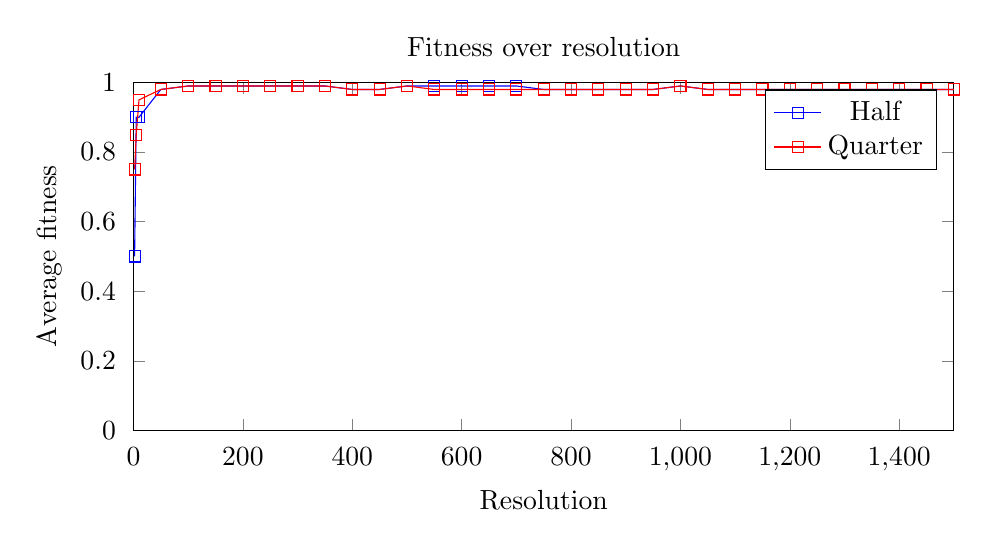
\begin{tikzpicture}
        \begin{axis}[
            width=12cm,
            height=6cm,
            title={Fitness over resolution},
            xlabel={Resolution},
            ylabel={Average fitness},
            enlargelimits=false,
            xmin=0,
            ymin=0, ymax=1,
            ytick={0,0.2,...,1},
            xticklabel shift={.1cm},
            yticklabel shift={.1cm} ]
        ]

        \addplot[
            color=blue,
            mark=square,
            ]
            coordinates {
                (2,0.50)(5,0.90)(10,0.90)(50,0.98)(100,0.99)(150,0.99)(200,0.99)(250,0.99)(300,0.99)(350,0.99)(400,0.98)(450,0.98)(500,0.99)(550,0.99)(600,0.99)(650,0.99)(700,0.99)(750,0.98)(800,0.98)(850,0.98)(900,0.98)(950,0.98)(1000,0.99)(1050,0.98)(1100,0.98)(1150,0.98)(1200,0.98)(1250,0.98)(1300,0.98)(1350,0.98)(1400,0.98)(1450,0.98)(1500,0.98)
            };
            \addlegendentry{Half}
        \addplot[
            color=red,
            mark=square,
            ]
            coordinates {
                (2,0.75)(5,0.85)(10,0.95)(50,0.98)(100,0.99)(150,0.99)(200,0.99)(250,0.99)(300,0.99)(350,0.99)(400,0.98)(450,0.98)(500,0.99)(550,0.98)(600,0.98)(650,0.98)(700,0.98)(750,0.98)(800,0.98)(850,0.98)(900,0.98)(950,0.98)(1000,0.99)(1050,0.98)(1100,0.98)(1150,0.98)(1200,0.98)(1250,0.98)(1300,0.98)(1350,0.98)(1400,0.98)(1450,0.98)(1500,0.98)
            };
            \addlegendentry{Quarter}
        \end{axis}
        \end{tikzpicture}
        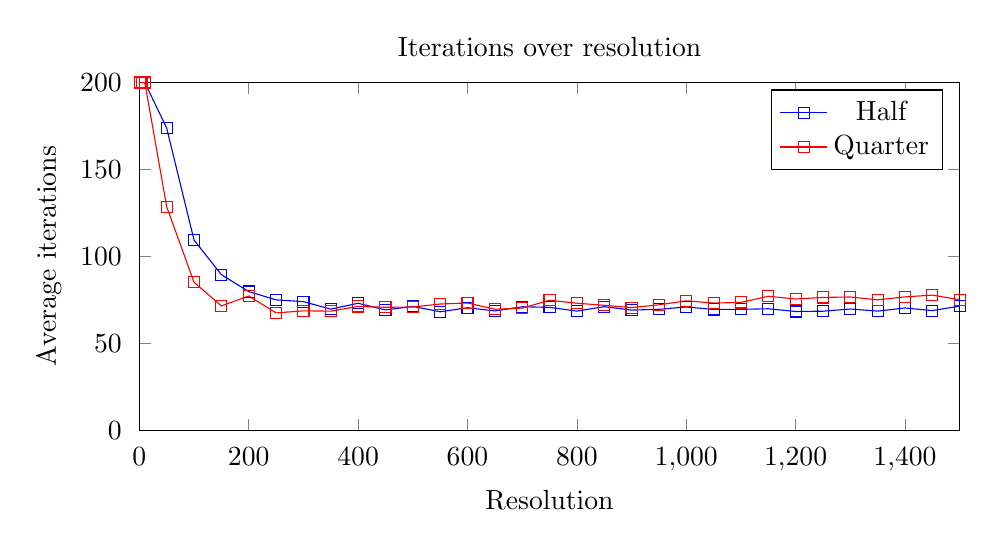
\begin{tikzpicture}
        \begin{axis}[
            width=12cm,
            height=6cm,
            title={Iterations over resolution},
            xlabel={Resolution},
            ylabel={Average iterations},
            xmin=0,
            ymin=0,
            enlargelimits=false,
            xticklabel shift={.1cm},
            yticklabel shift={.1cm} ]
        ]

        \addplot[
            color=blue,
            mark=square,
            ]
            coordinates {
                (2,200.00)(5,200.00)(10,200.00)(50,173.75)(100,109.39)(150,89.55)(200,79.81)(250,75.03)(300,74.03)(350,69.72)(400,73.08)(450,69.26)(500,71.27)(550,68.19)(600,70.51)(650,68.69)(700,71.07)(750,70.74)(800,68.57)(850,71.13)(900,69.16)(950,69.63)(1000,70.95)(1050,69.54)(1100,69.62)(1150,69.92)(1200,68.36)(1250,68.52)(1300,69.78)(1350,68.57)(1400,70.38)(1450,68.86)(1500,71.47)
            };
            \addlegendentry{Half}
        \addplot[
            color=red,
            mark=square,
            ]
            coordinates {
                (2,200.00)(5,200.00)(10,200.00)(50,128.58)(100,85.14)(150,71.56)(200,77.29)(250,67.54)(300,68.72)(350,68.57)(400,71.26)(450,70.78)(500,70.92)(550,72.64)(600,73.26)(650,69.66)(700,70.31)(750,74.80)(800,73.12)(850,71.89)(900,70.59)(950,72.19)(1000,74.49)(1050,73.20)(1100,73.56)(1150,77.10)(1200,75.52)(1250,76.44)(1300,76.69)(1350,75.07)(1400,76.75)(1450,77.77)(1500,75.14)
            };
            \addlegendentry{Quarter}
        \end{axis}
        \end{tikzpicture}
        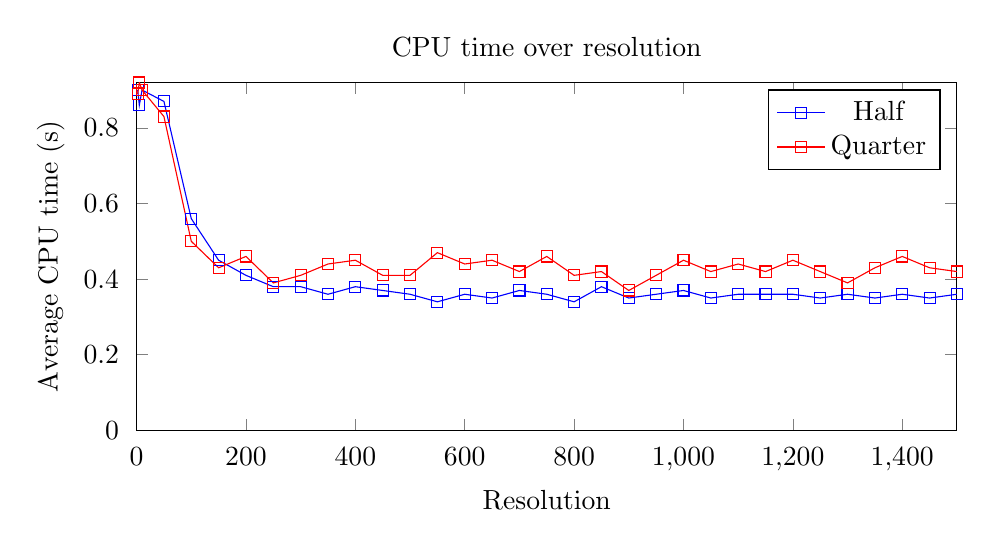
\begin{tikzpicture}
        \begin{axis}[
            width=12cm,
            height=6cm,
            title={CPU time over resolution},
            xlabel={Resolution},
            ylabel={Average CPU time (s)},
            xmin=0,
            ymin=0,
            enlargelimits=false,
            xticklabel shift={.1cm},
            yticklabel shift={.1cm} ]
        ]

        \addplot[
            color=blue,
            mark=square,
            ]
            coordinates {
                (2,0.90)(5,0.86)(10,0.90)(50,0.87)(100,0.56)(150,0.45)(200,0.41)(250,0.38)(300,0.38)(350,0.36)(400,0.38)(450,0.37)(500,0.36)(550,0.34)(600,0.36)(650,0.35)(700,0.37)(750,0.36)(800,0.34)(850,0.38)(900,0.35)(950,0.36)(1000,0.37)(1050,0.35)(1100,0.36)(1150,0.36)(1200,0.36)(1250,0.35)(1300,0.36)(1350,0.35)(1400,0.36)(1450,0.35)(1500,0.36)
            };
            \addlegendentry{Half}
        \addplot[
            color=red,
            mark=square,
            ]
            coordinates {
                (2,0.89)(5,0.92)(10,0.90)(50,0.83)(100,0.50)(150,0.43)(200,0.46)(250,0.39)(300,0.41)(350,0.44)(400,0.45)(450,0.41)(500,0.41)(550,0.47)(600,0.44)(650,0.45)(700,0.42)(750,0.46)(800,0.41)(850,0.42)(900,0.37)(950,0.41)(1000,0.45)(1050,0.42)(1100,0.44)(1150,0.42)(1200,0.45)(1250,0.42)(1300,0.39)(1350,0.43)(1400,0.46)(1450,0.43)(1500,0.42)
            };
            \addlegendentry{Quarter}
        \end{axis}
        \end{tikzpicture}
    \end{center}
    \caption{Performance metrics of the $(1 + 1)$ NA algorithm on the \textit{Half} and \texit{Quarter} benchmarks, with a single neuron, over different resolutions.
    The evolution stopped when the fitness was $2\%$ away from the maximal fitness of $1.0$. The maximum number of iterations was set to $200$.}
    \label{fig:na_maxiter}
\end{figure}

\begin{figure}
    \begin{center}
        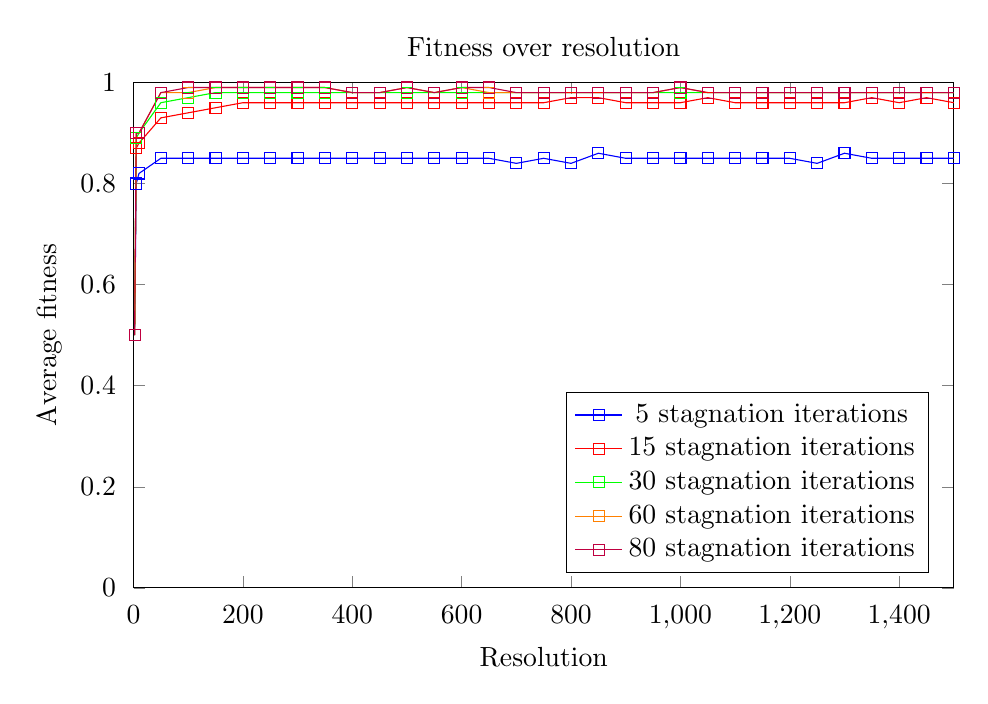
\begin{tikzpicture}
        \begin{axis}[
            width=12cm,
            height=8cm,
            title={Fitness over resolution},
            xlabel={Resolution},
            ylabel={Average fitness},
            enlargelimits=false,
            legend pos=south east,
            xmin=0,
            ymin=0, ymax=1,
            ytick={0,0.2,...,1},
            xticklabel shift={.1cm},
            yticklabel shift={.1cm} ]
        ]

        \addplot[
            color=blue,
            mark=square,
            ]
            coordinates {
                (2,0.50)(5,0.80)(10,0.82)(50,0.85)(100,0.85)(150,0.85)(200,0.85)(250,0.85)(300,0.85)(350,0.85)(400,0.85)(450,0.85)(500,0.85)(550,0.85)(600,0.85)(650,0.85)(700,0.84)(750,0.85)(800,0.84)(850,0.86)(900,0.85)(950,0.85)(1000,0.85)(1050,0.85)(1100,0.85)(1150,0.85)(1200,0.85)(1250,0.84)(1300,0.86)(1350,0.85)(1400,0.85)(1450,0.85)(1500,0.85)
            };
            \addlegendentry{5 stagnation iterations}
        \addplot[
            color=red,
            mark=square,
            ]
            coordinates {
                (2,0.50)(5,0.87)(10,0.88)(50,0.93)(100,0.94)(150,0.95)(200,0.96)(250,0.96)(300,0.96)(350,0.96)(400,0.96)(450,0.96)(500,0.96)(550,0.96)(600,0.96)(650,0.96)(700,0.96)(750,0.96)(800,0.97)(850,0.97)(900,0.96)(950,0.96)(1000,0.96)(1050,0.97)(1100,0.96)(1150,0.96)(1200,0.96)(1250,0.96)(1300,0.96)(1350,0.97)(1400,0.96)(1450,0.97)(1500,0.96)
            };
            \addlegendentry{15 stagnation iterations}
        \addplot[
            color=green,
            mark=square,
            ]
            coordinates {
                (2,0.50)(5,0.89)(10,0.90)(50,0.96)(100,0.97)(150,0.98)(200,0.98)(250,0.98)(300,0.98)(350,0.98)(400,0.98)(450,0.98)(500,0.98)(550,0.98)(600,0.98)(650,0.98)(700,0.98)(750,0.98)(800,0.98)(850,0.98)(900,0.98)(950,0.98)(1000,0.98)(1050,0.98)(1100,0.98)(1150,0.98)(1200,0.98)(1250,0.98)(1300,0.98)(1350,0.98)(1400,0.98)(1450,0.98)(1500,0.98)
            };
            \addlegendentry{30 stagnation iterations}
        \addplot[
            color=orange,
            mark=square,
            ]
            coordinates {
                (2,0.50)(5,0.90)(10,0.90)(50,0.98)(100,0.98)(150,0.99)(200,0.99)(250,0.99)(300,0.99)(350,0.99)(400,0.98)(450,0.98)(500,0.99)(550,0.98)(600,0.99)(650,0.98)(700,0.98)(750,0.98)(800,0.98)(850,0.98)(900,0.98)(950,0.98)(1000,0.99)(1050,0.98)(1100,0.98)(1150,0.98)(1200,0.98)(1250,0.98)(1300,0.98)(1350,0.98)(1400,0.98)(1450,0.98)(1500,0.98)
            };
            \addlegendentry{60 stagnation iterations}
        \addplot[
            color=purple,
            mark=square,
            ]
            coordinates {
                (2,0.50)(5,0.90)(10,0.90)(50,0.98)(100,0.99)(150,0.99)(200,0.99)(250,0.99)(300,0.99)(350,0.99)(400,0.98)(450,0.98)(500,0.99)(550,0.98)(600,0.99)(650,0.99)(700,0.98)(750,0.98)(800,0.98)(850,0.98)(900,0.98)(950,0.98)(1000,0.99)(1050,0.98)(1100,0.98)(1150,0.98)(1200,0.98)(1250,0.98)(1300,0.98)(1350,0.98)(1400,0.98)(1450,0.98)(1500,0.98)
            };
            \addlegendentry{80 stagnation iterations}
        \end{axis}
        \end{tikzpicture}
        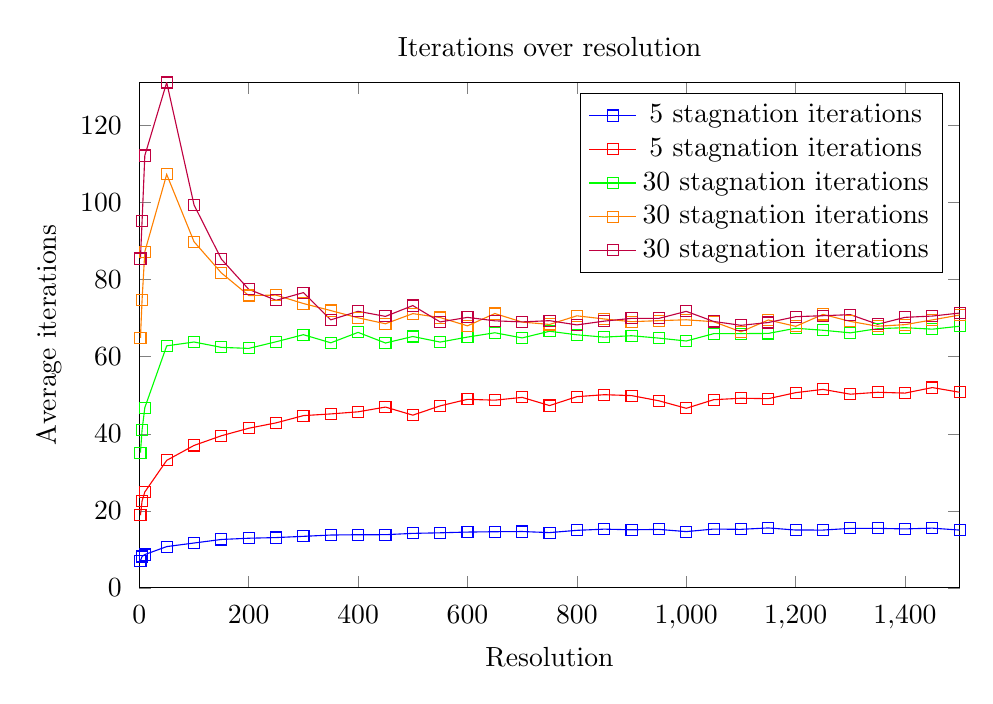
\begin{tikzpicture}
        \begin{axis}[
            width=12cm,
            height=8cm,
            title={Iterations over resolution},
            xlabel={Resolution},
            ylabel={Average iterations},
            xmin=0,
            ymin=0,
            enlargelimits=false,
            xticklabel shift={.1cm},
            yticklabel shift={.1cm} ]
        ]

        \addplot[
            color=blue,
            mark=square,
            ]
            coordinates {
                (2,7.06)(5,8.15)(10,8.65)(50,10.72)(100,11.65)(150,12.57)(200,12.89)(250,13.06)(300,13.38)(350,13.72)(400,13.80)(450,13.81)(500,14.15)(550,14.30)(600,14.49)(650,14.58)(700,14.63)(750,14.35)(800,14.94)(850,15.25)(900,15.08)(950,15.18)(1000,14.61)(1050,15.27)(1100,15.20)(1150,15.56)(1200,15.02)(1250,15.01)(1300,15.45)(1350,15.45)(1400,15.31)(1450,15.51)(1500,15.00)
            };
            \addlegendentry{5 stagnation iterations}
        \addplot[
            color=red,
            mark=square,
            ]
            coordinates {
                (2,18.86)(5,22.58)(10,24.90)(50,33.10)(100,36.98)(150,39.49)(200,41.44)(250,42.84)(300,44.72)(350,45.16)(400,45.71)(450,46.94)(500,44.84)(550,47.25)(600,48.95)(650,48.73)(700,49.45)(750,47.33)(800,49.64)(850,50.15)(900,49.92)(950,48.57)(1000,46.62)(1050,48.85)(1100,49.23)(1150,49.12)(1200,50.68)(1250,51.53)(1300,50.28)(1350,50.78)(1400,50.57)(1450,52.00)(1500,50.78)
            };
            \addlegendentry{5 stagnation iterations}
        \addplot[
            color=green,
            mark=square,
            ]
            coordinates {
                (2,35.10)(5,41.03)(10,46.80)(50,62.83)(100,63.83)(150,62.44)(200,62.17)(250,63.89)(300,65.73)(350,63.62)(400,66.33)(450,63.57)(500,65.26)(550,63.81)(600,65.11)(650,66.23)(700,64.89)(750,66.62)(800,65.70)(850,65.10)(900,65.46)(950,64.84)(1000,64.09)(1050,65.99)(1100,66.01)(1150,66.06)(1200,67.40)(1250,66.88)(1300,66.21)(1350,67.29)(1400,67.55)(1450,67.16)(1500,67.93)
            };
            \addlegendentry{30 stagnation iterations}
        \addplot[
            color=orange,
            mark=square,
            ]
            coordinates {
                (2,64.93)(5,74.80)(10,87.27)(50,107.34)(100,89.86)(150,81.76)(200,75.90)(250,75.99)(300,73.82)(350,71.99)(400,70.11)(450,68.57)(500,71.20)(550,70.18)(600,68.02)(650,71.22)(700,69.00)(750,68.39)(800,70.63)(850,69.81)(900,69.11)(950,69.37)(1000,69.60)(1050,69.10)(1100,66.48)(1150,69.54)(1200,67.90)(1250,70.99)(1300,69.18)(1350,67.92)(1400,68.34)(1450,69.57)(1500,70.84)
            };
            \addlegendentry{30 stagnation iterations}
        \addplot[
            color=purple,
            mark=square,
            ]
            coordinates {
                (2,85.50)(5,95.21)(10,112.23)(50,131.20)(100,99.42)(150,85.34)(200,77.51)(250,74.66)(300,76.65)(350,69.58)(400,71.80)(450,70.48)(500,73.29)(550,69.04)(600,70.22)(650,69.33)(700,69.05)(750,69.37)(800,68.27)(850,69.25)(900,69.97)(950,69.96)(1000,71.79)(1050,69.17)(1100,68.16)(1150,68.89)(1200,70.40)(1250,70.66)(1300,70.93)(1350,68.44)(1400,70.23)(1450,70.57)(1500,71.35)
            };
            \addlegendentry{30 stagnation iterations}
        \end{axis}
        \end{tikzpicture}
    \end{center}
    \caption{Performance metrics of the $(1 + 1)$ NA algorithm on the \textit{Half} benchmark, with a single neuron, over different resolutions.
    The evolution stopped when the fitness was $2\%$ away from the maximal fitness of $1.0$ or the maximum number of stagnation iteration was reached.}
    \label{fig:na_half_stagnation}
\end{figure}

\begin{figure}
    \begin{center}
        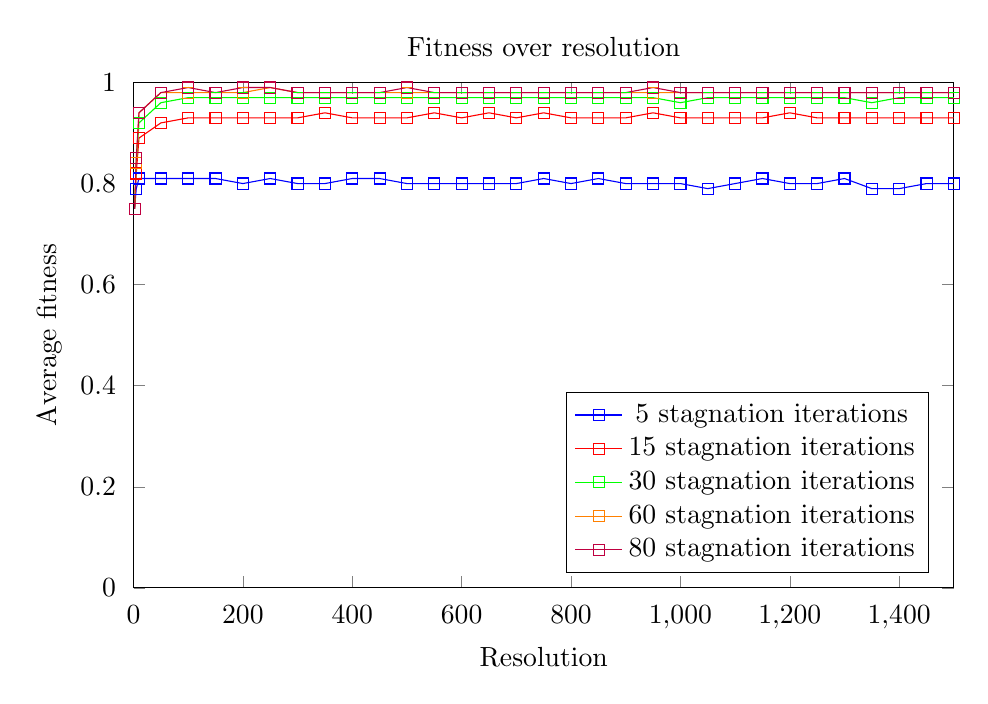
\begin{tikzpicture}
        \begin{axis}[
            width=12cm,
            height=8cm,
            title={Fitness over resolution},
            xlabel={Resolution},
            ylabel={Average fitness},
            enlargelimits=false,
            legend pos=south east,
            xmin=0,
            ymin=0, ymax=1,
            ytick={0,0.2,...,1},
            xticklabel shift={.1cm},
            yticklabel shift={.1cm} ]
        ]

        \addplot[
            color=blue,
            mark=square,
            ]
            coordinates {
                (2,0.75)(5,0.79)(10,0.81)(50,0.81)(100,0.81)(150,0.81)(200,0.80)(250,0.81)(300,0.80)(350,0.80)(400,0.81)(450,0.81)(500,0.80)(550,0.80)(600,0.80)(650,0.80)(700,0.80)(750,0.81)(800,0.80)(850,0.81)(900,0.80)(950,0.80)(1000,0.80)(1050,0.79)(1100,0.80)(1150,0.81)(1200,0.80)(1250,0.80)(1300,0.81)(1350,0.79)(1400,0.79)(1450,0.80)(1500,0.80)
            };
            \addlegendentry{5 stagnation iterations}
        \addplot[
            color=red,
            mark=square,
            ]
            coordinates {
                (2,0.75)(5,0.82)(10,0.89)(50,0.92)(100,0.93)(150,0.93)(200,0.93)(250,0.93)(300,0.93)(350,0.94)(400,0.93)(450,0.93)(500,0.93)(550,0.94)(600,0.93)(650,0.94)(700,0.93)(750,0.94)(800,0.93)(850,0.93)(900,0.93)(950,0.94)(1000,0.93)(1050,0.93)(1100,0.93)(1150,0.93)(1200,0.94)(1250,0.93)(1300,0.93)(1350,0.93)(1400,0.93)(1450,0.93)(1500,0.93)
            };
            \addlegendentry{15 stagnation iterations}
        \addplot[
            color=green,
            mark=square,
            ]
            coordinates {
                (2,0.75)(5,0.84)(10,0.92)(50,0.96)(100,0.97)(150,0.97)(200,0.97)(250,0.97)(300,0.97)(350,0.97)(400,0.97)(450,0.97)(500,0.97)(550,0.97)(600,0.97)(650,0.97)(700,0.97)(750,0.97)(800,0.97)(850,0.97)(900,0.97)(950,0.97)(1000,0.96)(1050,0.97)(1100,0.97)(1150,0.97)(1200,0.97)(1250,0.97)(1300,0.97)(1350,0.96)(1400,0.97)(1450,0.97)(1500,0.97)
            };
            \addlegendentry{30 stagnation iterations}
        \addplot[
            color=orange,
            mark=square,
            ]
            coordinates {
                (2,0.75)(5,0.84)(10,0.94)(50,0.98)(100,0.98)(150,0.98)(200,0.98)(250,0.99)(300,0.98)(350,0.98)(400,0.98)(450,0.98)(500,0.98)(550,0.98)(600,0.98)(650,0.98)(700,0.98)(750,0.98)(800,0.98)(850,0.98)(900,0.98)(950,0.98)(1000,0.98)(1050,0.98)(1100,0.98)(1150,0.98)(1200,0.98)(1250,0.98)(1300,0.98)(1350,0.98)(1400,0.98)(1450,0.98)(1500,0.98)
            };
            \addlegendentry{60 stagnation iterations}
        \addplot[
            color=purple,
            mark=square,
            ]
            coordinates {
                (2,0.75)(5,0.85)(10,0.94)(50,0.98)(100,0.99)(150,0.98)(200,0.99)(250,0.99)(300,0.98)(350,0.98)(400,0.98)(450,0.98)(500,0.99)(550,0.98)(600,0.98)(650,0.98)(700,0.98)(750,0.98)(800,0.98)(850,0.98)(900,0.98)(950,0.99)(1000,0.98)(1050,0.98)(1100,0.98)(1150,0.98)(1200,0.98)(1250,0.98)(1300,0.98)(1350,0.98)(1400,0.98)(1450,0.98)(1500,0.98)
            };
            \addlegendentry{80 stagnation iterations}
        \end{axis}
        \end{tikzpicture}
        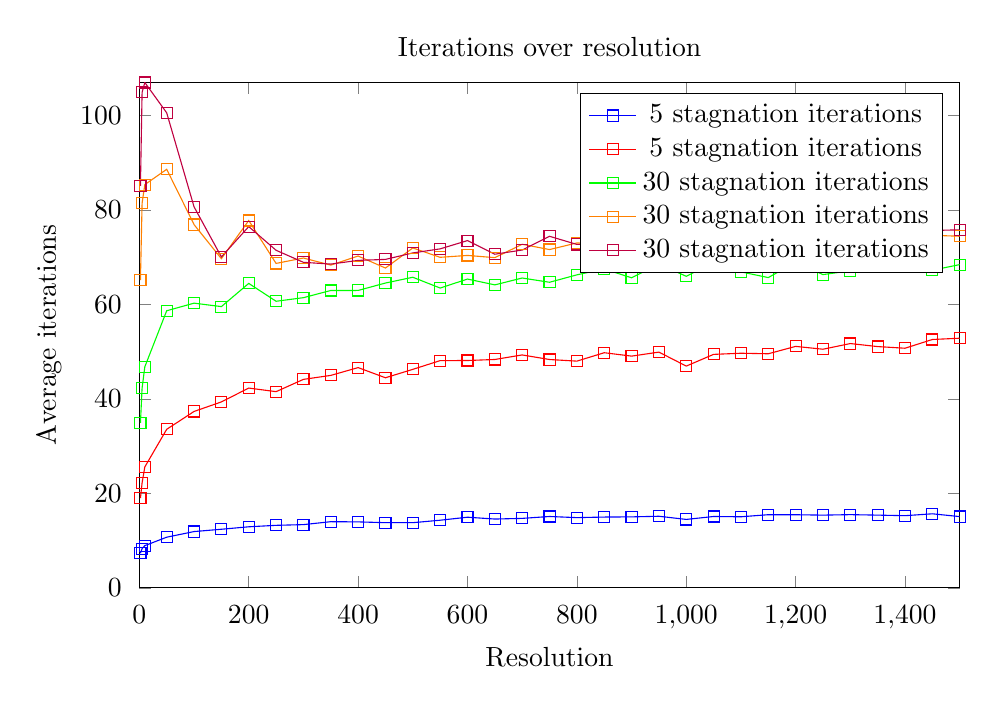
\begin{tikzpicture}
        \begin{axis}[
            width=12cm,
            height=8cm,
            title={Iterations over resolution},
            xlabel={Resolution},
            ylabel={Average iterations},
            xmin=0,
            ymin=0,
            enlargelimits=false,
            xticklabel shift={.1cm},
            yticklabel shift={.1cm} ]
        ]

        \addplot[
            color=blue,
            mark=square,
            ]
            coordinates {
                (2,7.32)(5,8.31)(10,8.94)(50,10.73)(100,11.92)(150,12.41)(200,12.93)(250,13.24)(300,13.39)(350,14.01)(400,13.97)(450,13.80)(500,13.80)(550,14.32)(600,14.96)(650,14.57)(700,14.71)(750,15.11)(800,14.87)(850,14.99)(900,15.03)(950,15.16)(1000,14.49)(1050,15.11)(1100,15.05)(1150,15.49)(1200,15.48)(1250,15.40)(1300,15.50)(1350,15.40)(1400,15.28)(1450,15.68)(1500,15.09)
            };
            \addlegendentry{5 stagnation iterations}
        \addplot[
            color=red,
            mark=square,
            ]
            coordinates {
                (2,19.01)(5,22.21)(10,25.60)(50,33.56)(100,37.34)(150,39.36)(200,42.29)(250,41.53)(300,44.13)(350,44.97)(400,46.62)(450,44.47)(500,46.25)(550,48.10)(600,48.12)(650,48.34)(700,49.30)(750,48.33)(800,47.99)(850,49.77)(900,49.05)(950,49.90)(1000,46.94)(1050,49.42)(1100,49.66)(1150,49.55)(1200,51.11)(1250,50.51)(1300,51.71)(1350,51.07)(1400,50.72)(1450,52.57)(1500,52.84)
            };
            \addlegendentry{5 stagnation iterations}
        \addplot[
            color=green,
            mark=square,
            ]
            coordinates {
                (2,34.90)(5,42.26)(10,46.79)(50,58.65)(100,60.26)(150,59.53)(200,64.44)(250,60.66)(300,61.42)(350,62.94)(400,62.95)(450,64.52)(500,65.74)(550,63.46)(600,65.36)(650,64.13)(700,65.58)(750,64.68)(800,66.25)(850,67.50)(900,65.62)(950,68.56)(1000,65.94)(1050,68.91)(1100,66.88)(1150,65.67)(1200,68.95)(1250,66.30)(1300,67.12)(1350,68.57)(1400,68.28)(1450,67.23)(1500,68.42)
            };
            \addlegendentry{30 stagnation iterations}
        \addplot[
            color=orange,
            mark=square,
            ]
            coordinates {
                (2,65.12)(5,81.40)(10,85.35)(50,88.59)(100,76.89)(150,69.67)(200,77.75)(250,68.67)(300,69.81)(350,68.31)(400,70.23)(450,67.69)(500,71.94)(550,69.96)(600,70.36)(650,69.89)(700,72.72)(750,71.60)(800,73.00)(850,72.79)(900,70.43)(950,72.85)(1000,73.94)(1050,73.24)(1100,71.88)(1150,70.81)(1200,73.85)(1250,72.48)(1300,72.25)(1350,72.97)(1400,74.65)(1450,74.62)(1500,74.42)
            };
            \addlegendentry{30 stagnation iterations}
        \addplot[
            color=purple,
            mark=square,
            ]
            coordinates {
                (2,85.07)(5,104.87)(10,106.96)(50,100.54)(100,80.65)(150,70.04)(200,76.46)(250,71.45)(300,68.90)(350,68.53)(400,69.31)(450,69.52)(500,70.89)(550,71.75)(600,73.50)(650,70.62)(700,71.50)(750,74.41)(800,72.69)(850,72.92)(900,73.98)(950,70.70)(1000,76.71)(1050,73.13)(1100,73.70)(1150,76.53)(1200,71.96)(1250,75.06)(1300,73.11)(1350,76.36)(1400,77.01)(1450,75.64)(1500,75.78)
            };
            \addlegendentry{30 stagnation iterations}
        \end{axis}
        \end{tikzpicture}
    \end{center}
    \caption{Performance metrics of the $(1 + 1)$ NA algorithm on the \textit{Quarter} benchmark, with a single neuron, over different resolutions.
    The evolution stopped when the fitness was $2\%$ away from the maximal fitness of $1.0$ or the maximum number of stagnation iteration was reached.}
    \label{fig:na_quarter_stagnation}
\end{figure}

\begin{figure}
    \begin{center}
        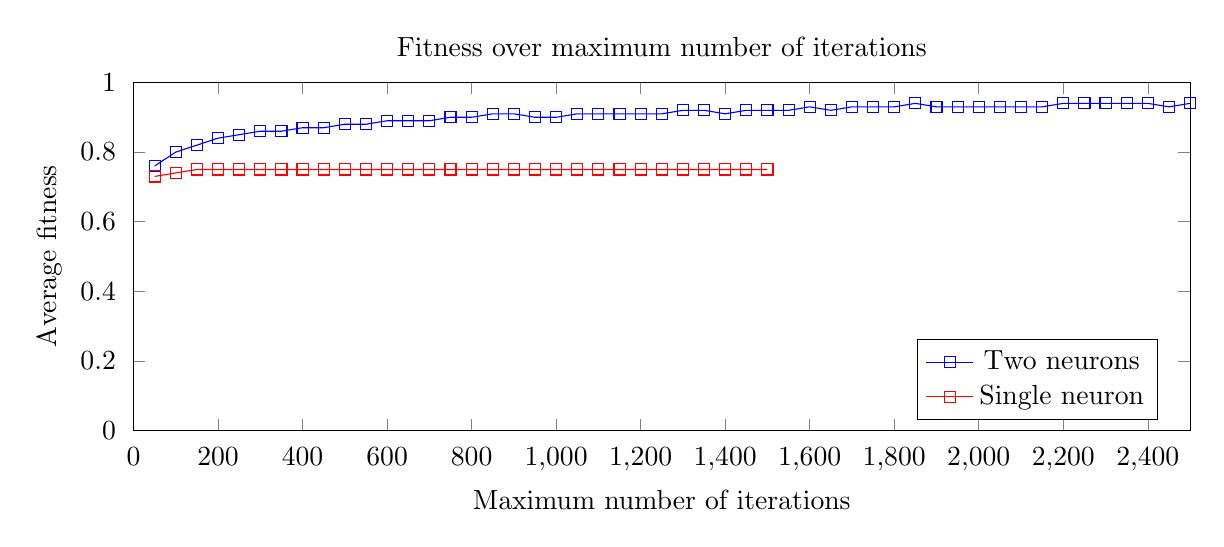
\begin{tikzpicture}
        \begin{axis}[
            width=15cm,
            height=6cm,
            title={Fitness over maximum number of iterations},
            legend pos=south east,
            xlabel={Maximum number of iterations},
            ylabel={Average fitness},
            enlargelimits=false,
            xmin=0,
            ymin=0, ymax=1,
            ytick={0,0.2,...,1},
            xticklabel shift={.1cm},
            yticklabel shift={.1cm} ]
        ]

        \addplot[
            color=blue,
            mark=square,
            ]
            coordinates {
                (50,0.76)(100,0.80)(150,0.82)(200,0.84)(250,0.85)(300,0.86)(350,0.86)(400,0.87)(450,0.87)(500,0.88)(550,0.88)(600,0.89)(650,0.89)(700,0.89)(750,0.90)(800,0.90)(850,0.91)(900,0.91)(950,0.90)(1000,0.90)(1050,0.91)(1100,0.91)(1150,0.91)(1200,0.91)(1250,0.91)(1300,0.92)(1350,0.92)(1400,0.91)(1450,0.92)(1500,0.92)(1550,0.92)(1600,0.93)(1650,0.92)(1700,0.93)(1750,0.93)(1800,0.93)(1850,0.94)(1900,0.93)(1950,0.93)(2000,0.93)(2050,0.93)(2100,0.93)(2150,0.93)(2200,0.94)(2250,0.94)(2300,0.94)(2350,0.94)(2400,0.94)(2450,0.93)(2500,0.94)
            };
            \addlegendentry{Two neurons}
        \addplot[
            color=red,
            mark=square,
            ]
            coordinates {
                (50,0.73)(100,0.74)(150,0.75)(200,0.75)(250,0.75)(300,0.75)(350,0.75)(400,0.75)(450,0.75)(500,0.75)(550,0.75)(600,0.75)(650,0.75)(700,0.75)(750,0.75)(800,0.75)(850,0.75)(900,0.75)(950,0.75)(1000,0.75)(1050,0.75)(1100,0.75)(1150,0.75)(1200,0.75)(1250,0.75)(1300,0.75)(1350,0.75)(1400,0.75)(1450,0.75)(1500,0.75)
            };
            \addlegendentry{Single neuron}
        \end{axis}
        \end{tikzpicture}
        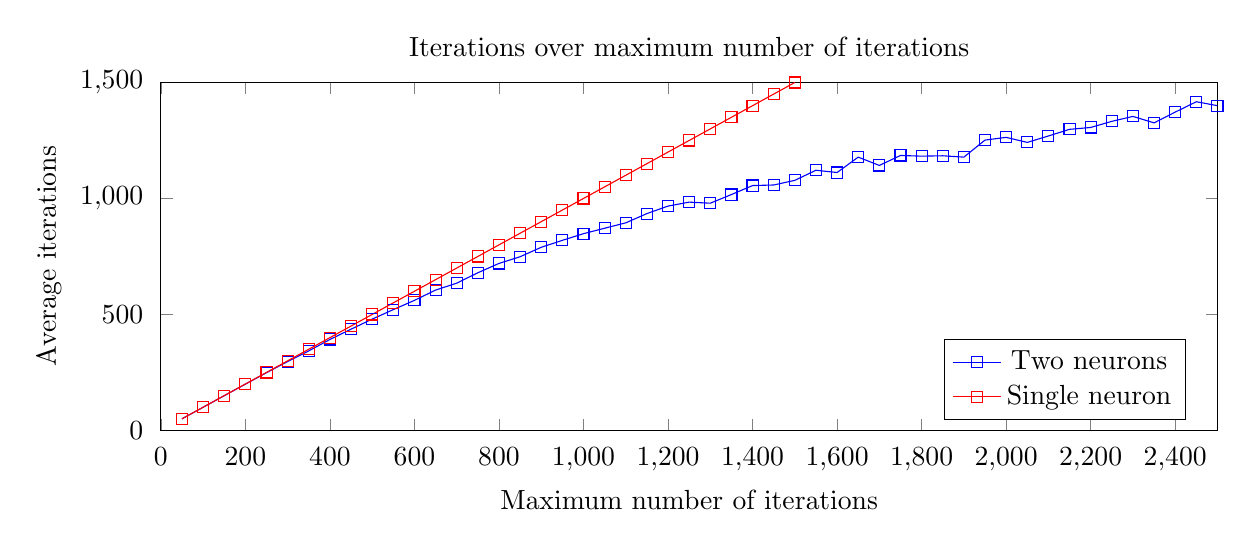
\begin{tikzpicture}
        \begin{axis}[
            width=15cm,
            height=6cm,
            legend pos=south east,
            title={Iterations over maximum number of iterations},
            xlabel={Maximum number of iterations},
            ylabel={Average iterations},
            xmin=0,
            ymin=0,
            enlargelimits=false,
            xticklabel shift={.1cm},
            yticklabel shift={.1cm} ]
        ]

        \addplot[
            color=blue,
            mark=square,
            ]
            coordinates {
                (50,49.97)(100,99.88)(150,149.73)(200,199.47)(250,248.90)(300,296.92)(350,342.93)(400,392.04)(450,436.46)(500,479.91)(550,520.86)(600,560.64)(650,604.99)(700,634.84)(750,679.66)(800,719.92)(850,748.80)(900,789.45)(950,819.47)(1000,848.19)(1050,871.68)(1100,894.90)(1150,934.78)(1200,967.18)(1250,984.16)(1300,979.59)(1350,1016.89)(1400,1055.63)(1450,1058.06)(1500,1078.15)(1550,1121.60)(1600,1111.85)(1650,1178.21)(1700,1142.42)(1750,1185.41)(1800,1182.37)(1850,1184.01)(1900,1178.17)(1950,1251.66)(2000,1263.44)(2050,1241.68)(2100,1269.41)(2150,1298.02)(2200,1306.06)(2250,1332.45)(2300,1353.79)(2350,1325.92)(2400,1372.23)(2450,1417.02)(2500,1400.06)
            };
            \addlegendentry{Two neurons}
        \addplot[
            color=red,
            mark=square,
            ]
            coordinates {
                (50,50.00)(100,100.00)(150,150.00)(200,200.00)(250,250.00)(300,300.00)(350,350.00)(400,400.00)(450,450.00)(500,500.00)(550,550.00)(600,600.00)(650,650.00)(700,700.00)(750,750.00)(800,800.00)(850,850.00)(900,900.00)(950,950.00)(1000,1000.00)(1050,1050.00)(1100,1100.00)(1150,1150.00)(1200,1200.00)(1250,1250.00)(1300,1300.00)(1350,1350.00)(1400,1400.00)(1450,1450.00)(1500,1500.00)
            };
            \addlegendentry{Single neuron}
        \end{axis}
        \end{tikzpicture}
        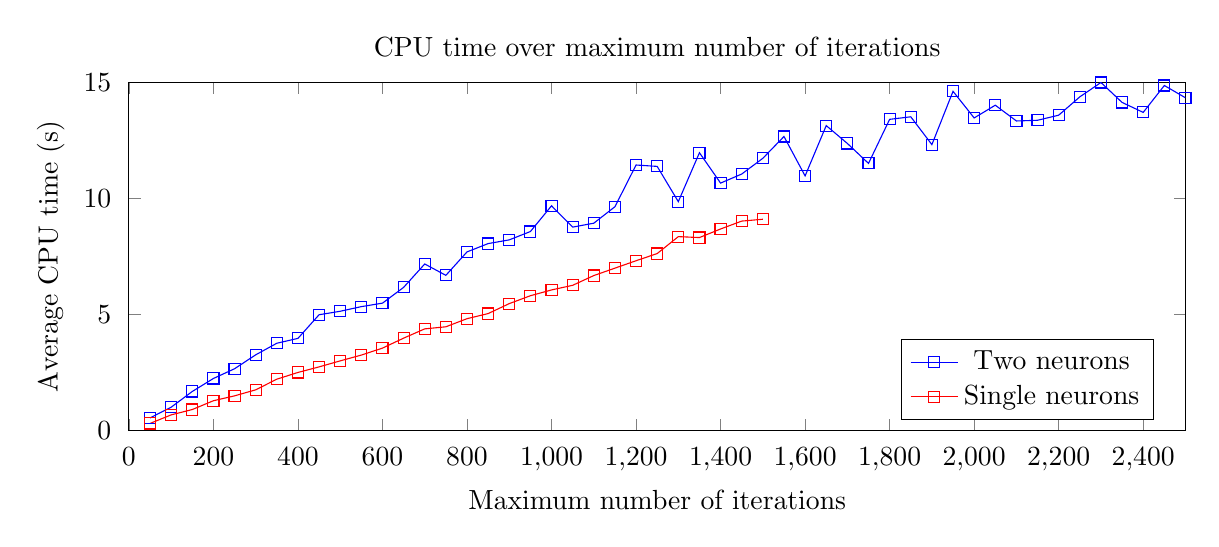
\begin{tikzpicture}
        \begin{axis}[
            width=15cm,
            height=6cm,
            legend pos=south east,
            title={CPU time over maximum number of iterations},
            xlabel={Maximum number of iterations},
            ylabel={Average CPU time (s)},
            xmin=0,
            ymin=0,
            enlargelimits=false,
            xticklabel shift={.1cm},
            yticklabel shift={.1cm} ]
        ]

        \addplot[
            color=blue,
            mark=square,
            ]
            coordinates {
                (50,0.54)(100,1.00)(150,1.68)(200,2.24)(250,2.66)(300,3.26)(350,3.76)(400,3.97)(450,4.99)(500,5.14)(550,5.34)(600,5.49)(650,6.17)(700,7.18)(750,6.69)(800,7.70)(850,8.06)(900,8.22)(950,8.58)(1000,9.69)(1050,8.77)(1100,8.94)(1150,9.65)(1200,11.45)(1250,11.39)(1300,9.87)(1350,11.98)(1400,10.67)(1450,11.06)(1500,11.74)(1550,12.68)(1600,10.98)(1650,13.15)(1700,12.38)(1750,11.52)(1800,13.42)(1850,13.53)(1900,12.33)(1950,14.63)(2000,13.48)(2050,14.03)(2100,13.35)(2150,13.38)(2200,13.60)(2250,14.39)(2300,15.01)(2350,14.15)(2400,13.72)(2450,14.88)(2500,14.35)
            };
            \addlegendentry{Two neurons}
        \addplot[
            color=red,
            mark=square,
            ]
            coordinates {
                (50,0.30)(100,0.67)(150,0.90)(200,1.28)(250,1.49)(300,1.75)(350,2.21)(400,2.50)(450,2.74)(500,3.00)(550,3.25)(600,3.55)(650,3.98)(700,4.38)(750,4.47)(800,4.82)(850,5.04)(900,5.47)(950,5.81)(1000,6.06)(1050,6.26)(1100,6.68)(1150,7.00)(1200,7.32)(1250,7.63)(1300,8.36)(1350,8.32)(1400,8.69)(1450,9.03)(1500,9.11)
            };
            \addlegendentry{Single neurons}
        \end{axis}
        \end{tikzpicture}
    \end{center}
    \caption{Performance metrics of the $(1 + 1)$ NA algorithm on the \textit{TwoQuarters} benchmark, over different maximum iterations.
    The evolution stopped when the fitness was $2\%$ away from the maximal fitness of $1.0$ or the maximum number of iterations was reached.}
    \label{fig:na_twoquarters}
\end{figure}

\begin{figure}
    \begin{center}
        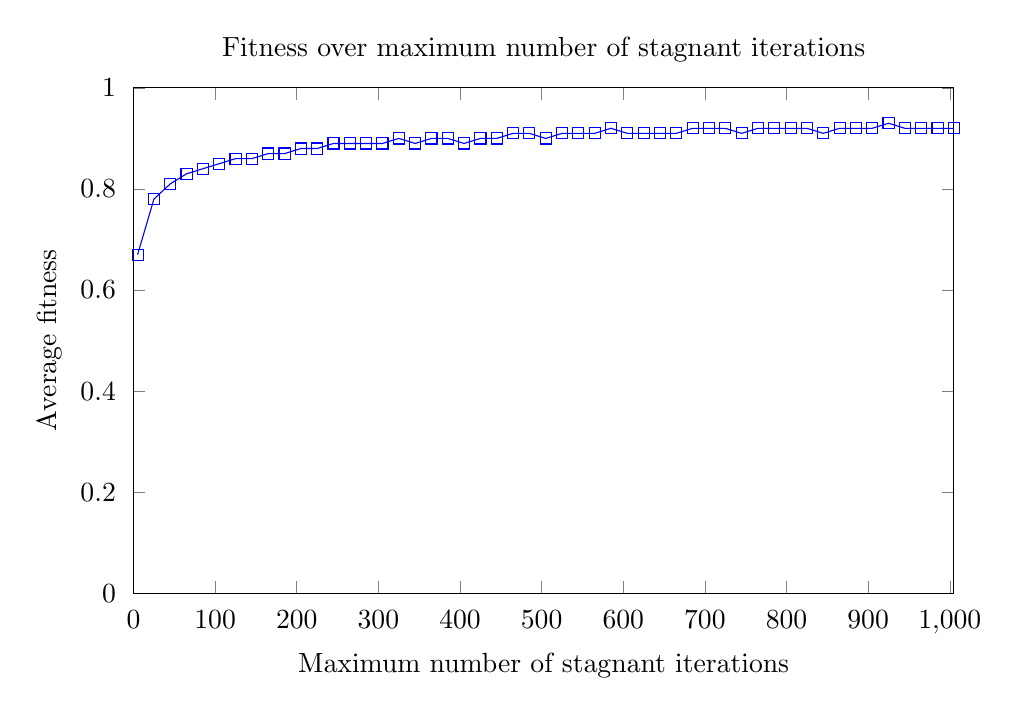
\begin{tikzpicture}
        \begin{axis}[
            width=12cm,
            height=8cm,
            title={Fitness over maximum number of stagnant iterations},
            xlabel={Maximum number of stagnant iterations},
            ylabel={Average fitness},
            enlargelimits=false,
            xmin=0,
            ymin=0, ymax=1,
            ytick={0,0.2,...,1},
            xticklabel shift={.1cm},
            yticklabel shift={.1cm} ]
        ]

        \addplot[
            color=blue,
            mark=square,
            ]
            coordinates {
                (5,0.67)(25,0.78)(45,0.81)(65,0.83)(85,0.84)(105,0.85)(125,0.86)(145,0.86)(165,0.87)(185,0.87)(205,0.88)(225,0.88)(245,0.89)(265,0.89)(285,0.89)(305,0.89)(325,0.90)(345,0.89)(365,0.90)(385,0.90)(405,0.89)(425,0.90)(445,0.90)(465,0.91)(485,0.91)(505,0.90)(525,0.91)(545,0.91)(565,0.91)(585,0.92)(605,0.91)(625,0.91)(645,0.91)(665,0.91)(685,0.92)(705,0.92)(725,0.92)(745,0.91)(765,0.92)(785,0.92)(805,0.92)(825,0.92)(845,0.91)(865,0.92)(885,0.92)(905,0.92)(925,0.93)(945,0.92)(965,0.92)(985,0.92)(1005,0.92)
            };
        \end{axis}
        \end{tikzpicture}
        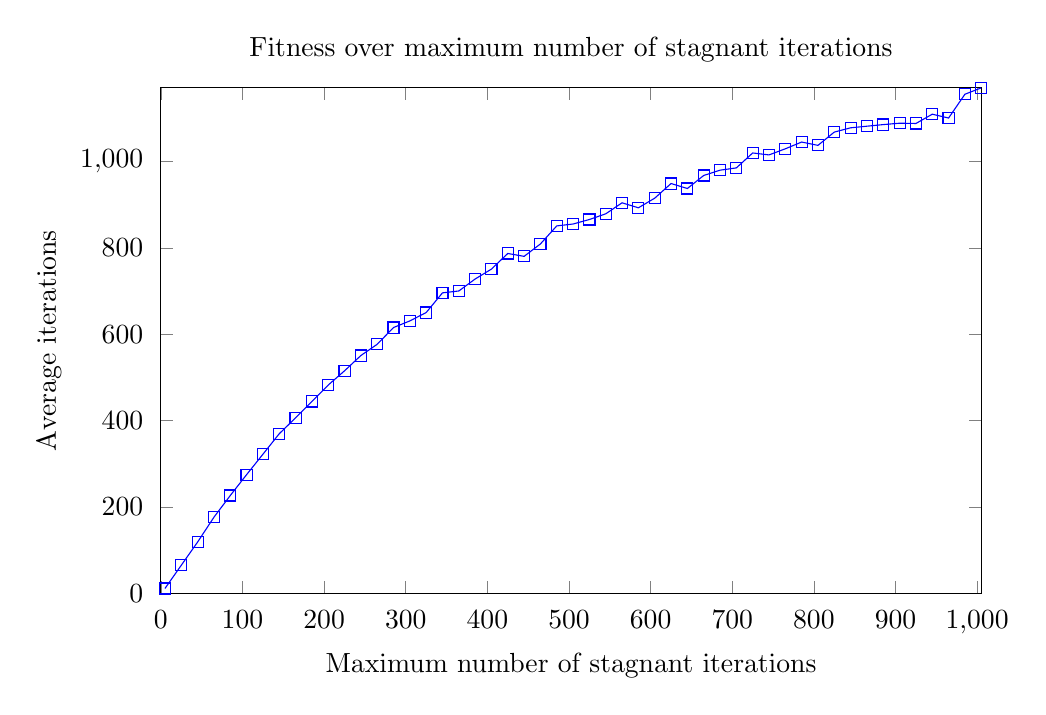
\begin{tikzpicture}
        \begin{axis}[
            width=12cm,
            height=8cm,
            title={Fitness over maximum number of stagnant iterations},
            xlabel={Maximum number of stagnant iterations},
            ylabel={Average iterations},
            xmin=0,
            ymin=0,
            enlargelimits=false,
            xticklabel shift={.1cm},
            yticklabel shift={.1cm} ]
        ]

        \addplot[
            color=blue,
            mark=square,
            ]
            coordinates {
                (5,11.08)(25,64.92)(45,118.66)(65,176.18)(85,226.47)(105,274.75)(125,322.09)(145,369.60)(165,406.29)(185,444.36)(205,482.35)(225,515.39)(245,550.76)(265,576.87)(285,615.67)(305,630.95)(325,650.39)(345,696.00)(365,700.34)(385,728.06)(405,751.11)(425,787.23)(445,780.55)(465,809.38)(485,851.13)(505,855.51)(525,865.96)(545,879.14)(565,904.62)(585,893.06)(605,915.34)(625,949.31)(645,937.78)(665,967.92)(685,980.22)(705,985.50)(725,1020.09)(745,1015.59)(765,1029.75)(785,1045.41)(805,1037.69)(825,1068.49)(845,1078.37)(865,1082.12)(885,1085.85)(905,1089.08)(925,1088.42)(945,1109.95)(965,1101.04)(985,1156.12)(1005,1170.91)
            };
        \end{axis}
        \end{tikzpicture}
    \end{center}
    \caption{Performance metrics of the $(1 + 1)$ NA algorithm on the \textit{TwoQuarters} benchmark with two  neurons, over different numbers of maximum stagnant iterations.
    The evolution stopped when the fitness was $2\%$ away from the maximal fitness of $1.0$, when $2500$ iterations was reached, or the maximum number of stagnant iterations was reached.}
    \label{fig:na_twoquarters_stag}
\end{figure}

\begin{figure}
    \begin{center}
        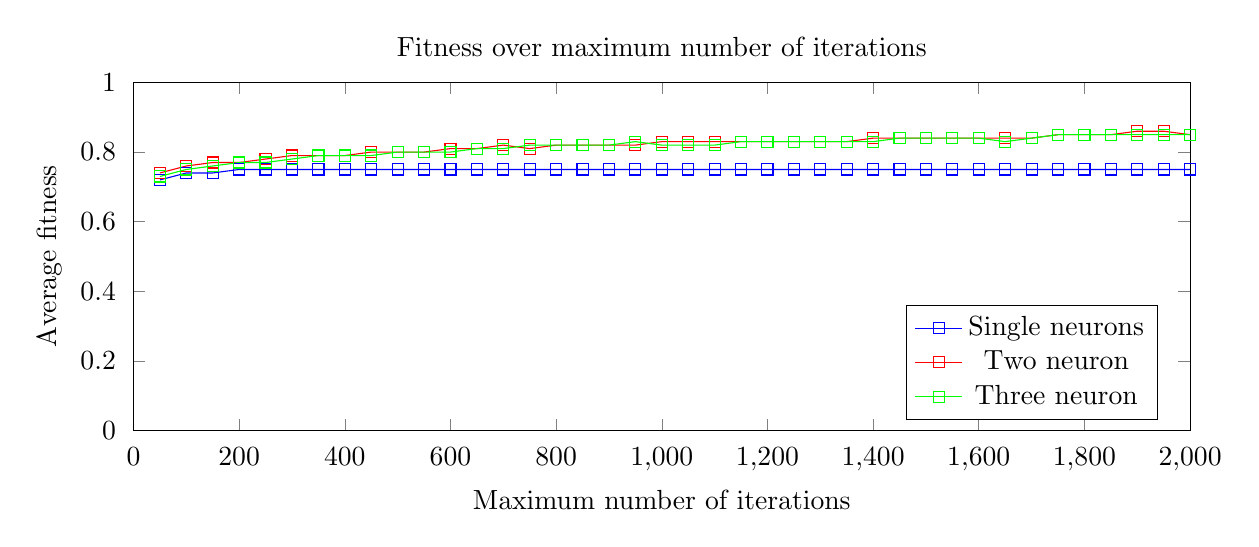
\begin{tikzpicture}
        \begin{axis}[
            width=15cm,
            height=6cm,
            title={Fitness over maximum number of iterations},
            legend pos=south east,
            xlabel={Maximum number of iterations},
            ylabel={Average fitness},
            enlargelimits=false,
            xmin=0,
            ymin=0, ymax=1,
            ytick={0,0.2,...,1},
            xticklabel shift={.1cm},
            yticklabel shift={.1cm} ]
        ]

        \addplot[
            color=blue,
            mark=square,
            ]
            coordinates {
                (50,0.72)(100,0.74)(150,0.74)(200,0.75)(250,0.75)(300,0.75)(350,0.75)(400,0.75)(450,0.75)(500,0.75)(550,0.75)(600,0.75)(650,0.75)(700,0.75)(750,0.75)(800,0.75)(850,0.75)(900,0.75)(950,0.75)(1000,0.75)(1050,0.75)(1100,0.75)(1150,0.75)(1200,0.75)(1250,0.75)(1300,0.75)(1350,0.75)(1400,0.75)(1450,0.75)(1500,0.75)(1550,0.75)(1600,0.75)(1650,0.75)(1700,0.75)(1750,0.75)(1800,0.75)(1850,0.75)(1900,0.75)(1950,0.75)(2000,0.75)
            };
            \addlegendentry{Single neurons}
        \addplot[
            color=red,
            mark=square,
            ]
            coordinates {
                (50,0.74)(100,0.76)(150,0.77)(200,0.77)(250,0.78)(300,0.79)(350,0.79)(400,0.79)(450,0.80)(500,0.80)(550,0.80)(600,0.81)(650,0.81)(700,0.82)(750,0.81)(800,0.82)(850,0.82)(900,0.82)(950,0.82)(1000,0.83)(1050,0.83)(1100,0.83)(1150,0.83)(1200,0.83)(1250,0.83)(1300,0.83)(1350,0.83)(1400,0.84)(1450,0.84)(1500,0.84)(1550,0.84)(1600,0.84)(1650,0.84)(1700,0.84)(1750,0.85)(1800,0.85)(1850,0.85)(1900,0.86)(1950,0.86)(2000,0.85)
            };
            \addlegendentry{Two neuron}
        \addplot[
            color=green,
            mark=square,
            ]
            coordinates {
                (50,0.73)(100,0.75)(150,0.76)(200,0.77)(250,0.77)(300,0.78)(350,0.79)(400,0.79)(450,0.79)(500,0.80)(550,0.80)(600,0.80)(650,0.81)(700,0.81)(750,0.82)(800,0.82)(850,0.82)(900,0.82)(950,0.83)(1000,0.82)(1050,0.82)(1100,0.82)(1150,0.83)(1200,0.83)(1250,0.83)(1300,0.83)(1350,0.83)(1400,0.83)(1450,0.84)(1500,0.84)(1550,0.84)(1600,0.84)(1650,0.83)(1700,0.84)(1750,0.85)(1800,0.85)(1850,0.85)(1900,0.85)(1950,0.85)(2000,0.85)
            };
            \addlegendentry{Three neuron}
        \end{axis}
        \end{tikzpicture}
        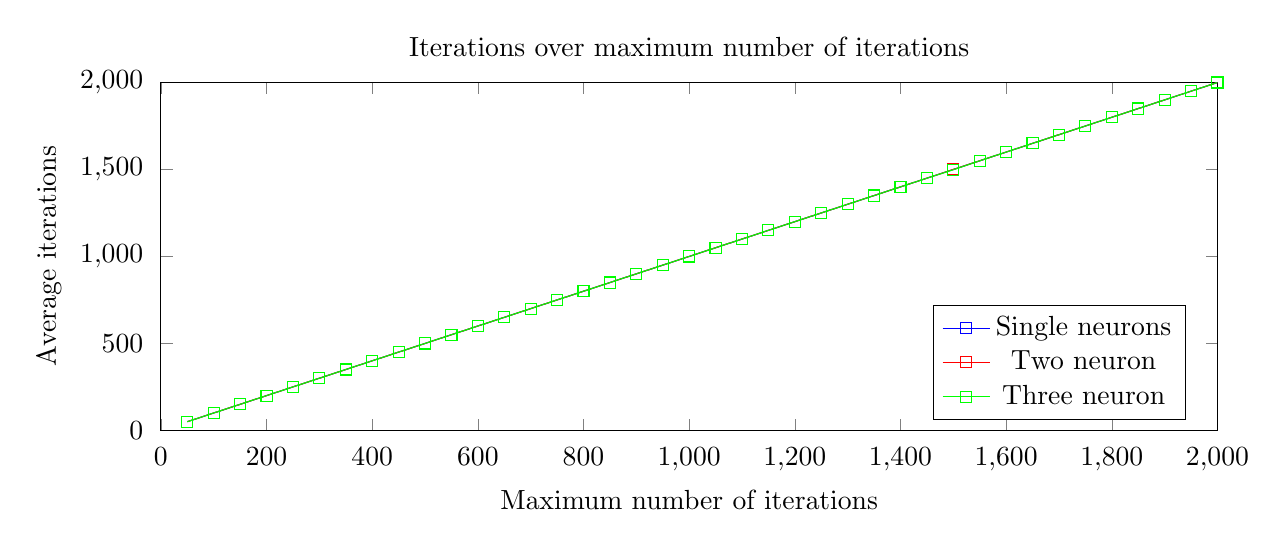
\begin{tikzpicture}
        \begin{axis}[
            width=15cm,
            height=6cm,
            legend pos=south east,
            title={Iterations over maximum number of iterations},
            xlabel={Maximum number of iterations},
            ylabel={Average iterations},
            xmin=0,
            ymin=0,
            enlargelimits=false,
            xticklabel shift={.1cm},
            yticklabel shift={.1cm} ]
        ]

        \addplot[
            color=blue,
            mark=square,
            ]
            coordinates {
                (50,50.00)(100,100.00)(150,150.00)(200,200.00)(250,250.00)(300,300.00)(350,350.00)(400,400.00)(450,450.00)(500,500.00)(550,550.00)(600,600.00)(650,650.00)(700,700.00)(750,750.00)(800,800.00)(850,850.00)(900,900.00)(950,950.00)(1000,1000.00)(1050,1050.00)(1100,1100.00)(1150,1150.00)(1200,1200.00)(1250,1250.00)(1300,1300.00)(1350,1350.00)(1400,1400.00)(1450,1450.00)(1500,1500.00)(1550,1550.00)(1600,1600.00)(1650,1650.00)(1700,1700.00)(1750,1750.00)(1800,1800.00)(1850,1850.00)(1900,1900.00)(1950,1950.00)(2000,2000.00)
            };
            \addlegendentry{Single neurons}
        \addplot[
            color=red,
            mark=square,
            ]
            coordinates {
                (50,50.00)(100,100.00)(150,150.00)(200,200.00)(250,250.00)(300,300.00)(350,350.00)(400,400.00)(450,450.00)(500,500.00)(550,550.00)(600,600.00)(650,650.00)(700,700.00)(750,750.00)(800,800.00)(850,850.00)(900,900.00)(950,950.00)(1000,1000.00)(1050,1050.00)(1100,1100.00)(1150,1150.00)(1200,1200.00)(1250,1250.00)(1300,1300.00)(1350,1350.00)(1400,1400.00)(1450,1450.00)(1500,1500.00)(1550,1550.00)(1600,1600.00)(1650,1650.00)(1700,1700.00)(1750,1750.00)(1800,1800.00)(1850,1850.00)(1900,1900.00)(1950,1950.00)(2000,2000.00)
            };
            \addlegendentry{Two neuron}
        \addplot[
            color=green,
            mark=square,
            ]
            coordinates {
                (50,50.00)(100,100.00)(150,150.00)(200,200.00)(250,250.00)(300,300.00)(350,350.00)(400,400.00)(450,450.00)(500,500.00)(550,550.00)(600,600.00)(650,650.00)(700,700.00)(750,750.00)(800,800.00)(850,850.00)(900,900.00)(950,950.00)(1000,1000.00)(1050,1050.00)(1100,1100.00)(1150,1150.00)(1200,1200.00)(1250,1250.00)(1300,1300.00)(1350,1350.00)(1400,1400.00)(1450,1450.00)(1500,1498.40)(1550,1550.00)(1600,1600.00)(1650,1650.00)(1700,1700.00)(1750,1750.00)(1800,1800.00)(1850,1850.00)(1900,1900.00)(1950,1950.00)(2000,2000.00)
            };
            \addlegendentry{Three neuron}
        \end{axis}
        \end{tikzpicture}
        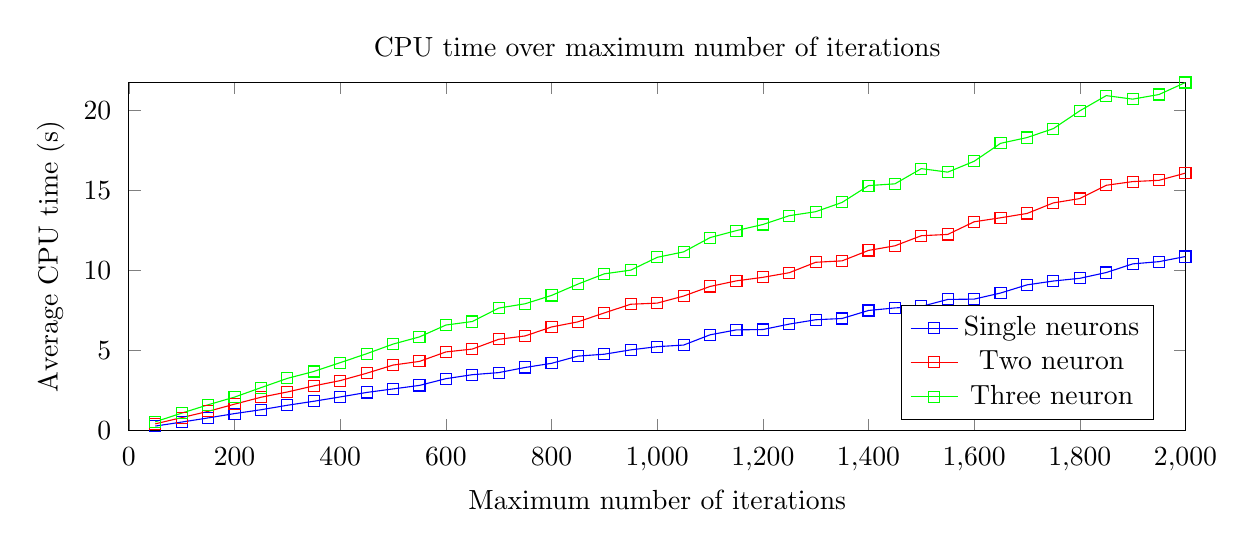
\begin{tikzpicture}
        \begin{axis}[
            width=15cm,
            height=6cm,
            legend pos=south east,
            title={CPU time over maximum number of iterations},
            xlabel={Maximum number of iterations},
            ylabel={Average CPU time (s)},
            xmin=0,
            ymin=0,
            enlargelimits=false,
            xticklabel shift={.1cm},
            yticklabel shift={.1cm} ]
        ]

        \addplot[
            color=blue,
            mark=square,
            ]
            coordinates {
                (50,0.27)(100,0.52)(150,0.78)(200,1.05)(250,1.29)(300,1.57)(350,1.82)(400,2.09)(450,2.37)(500,2.59)(550,2.81)(600,3.23)(650,3.48)(700,3.61)(750,3.93)(800,4.19)(850,4.64)(900,4.76)(950,5.03)(1000,5.23)(1050,5.33)(1100,5.97)(1150,6.28)(1200,6.30)(1250,6.64)(1300,6.91)(1350,6.99)(1400,7.49)(1450,7.65)(1500,7.74)(1550,8.18)(1600,8.20)(1650,8.58)(1700,9.09)(1750,9.33)(1800,9.50)(1850,9.86)(1900,10.40)(1950,10.54)(2000,10.86)
            };
            \addlegendentry{Single neurons}
        \addplot[
            color=red,
            mark=square,
            ]
            coordinates {
                (50,0.41)(100,0.80)(150,1.19)(200,1.64)(250,2.07)(300,2.40)(350,2.78)(400,3.11)(450,3.57)(500,4.08)(550,4.31)(600,4.90)(650,5.08)(700,5.69)(750,5.90)(800,6.46)(850,6.78)(900,7.34)(950,7.88)(1000,7.95)(1050,8.39)(1100,8.99)(1150,9.34)(1200,9.56)(1250,9.85)(1300,10.50)(1350,10.59)(1400,11.24)(1450,11.53)(1500,12.16)(1550,12.24)(1600,13.03)(1650,13.28)(1700,13.55)(1750,14.21)(1800,14.48)(1850,15.31)(1900,15.54)(1950,15.62)(2000,16.07)
            };
            \addlegendentry{Two neuron}
        \addplot[
            color=green,
            mark=square,
            ]
            coordinates {
                (50,0.54)(100,1.08)(150,1.60)(200,2.08)(250,2.67)(300,3.25)(350,3.68)(400,4.23)(450,4.79)(500,5.39)(550,5.84)(600,6.58)(650,6.80)(700,7.64)(750,7.91)(800,8.43)(850,9.14)(900,9.78)(950,10.01)(1000,10.81)(1050,11.15)(1100,12.04)(1150,12.48)(1200,12.86)(1250,13.41)(1300,13.66)(1350,14.24)(1400,15.29)(1450,15.40)(1500,16.35)(1550,16.13)(1600,16.81)(1650,17.93)(1700,18.29)(1750,18.85)(1800,19.96)(1850,20.91)(1900,20.69)(1950,20.98)(2000,21.73)
            };
            \addlegendentry{Three neuron}
        \end{axis}
        \end{tikzpicture}
    \end{center}
    \caption{Performance metrics of the $(1 + 1)$ NA algorithm on the \textit{LocalOpt} benchmark, over different maximum iterations.
    The evolution stopped when the fitness was $2\%$ away from the maximal fitness of $1.0$ or the maximum number of iterations was reached.}
    \label{fig:na_localopt}
\end{figure}

\subsubsection{Proben1 classification problem}

...

\subsection{Results of the BNA algorithm}

The BNA algorithm can be applied to binary classification problems. As it is the case for the $(1 + 1)$ NA algorithm, the BNA algorithm was tested on the spere classification problems,
the \textit{XOR} problem and the \textit{Cancer1} classification problem. The parameters which can be tuned for this algorithm are the resolution and the number of V-neurons,
Varying the resolution would simply highlight the same properties as the ones observed for the $(1 + 1)$ NA algorithm. Thus the focus will be on the number of V-neurons and the parameters
for the evolution of the algorithm. For the following experiments, the resolution was set to $400$.

\subsubsection{Unit-sphere classification problems}

The first experiment consisted in testing the algorithm on the \textit{Half} and \textit{Quarter} benchmarks. The results are shown in Figure \ref{fig:bna_half_quarter}. The algorithm
was tested with a maximum number of iterations ranging from $5$ to $300$. The evolution stopped when the fitness was $2\%$ away from the maximal fitness of $1.0$ or the maximum number
of iterations was reached. It can be seen that the number of iterations taken by the algorithm plateaus around $110$ iterations. Furthermore, as it was the case for the $(1 + 1)$ NA
algorithm, it can be seen on the graphs how the CPU time is proportional to the number of iterations.

...

\begin{figure}
    \begin{center}
        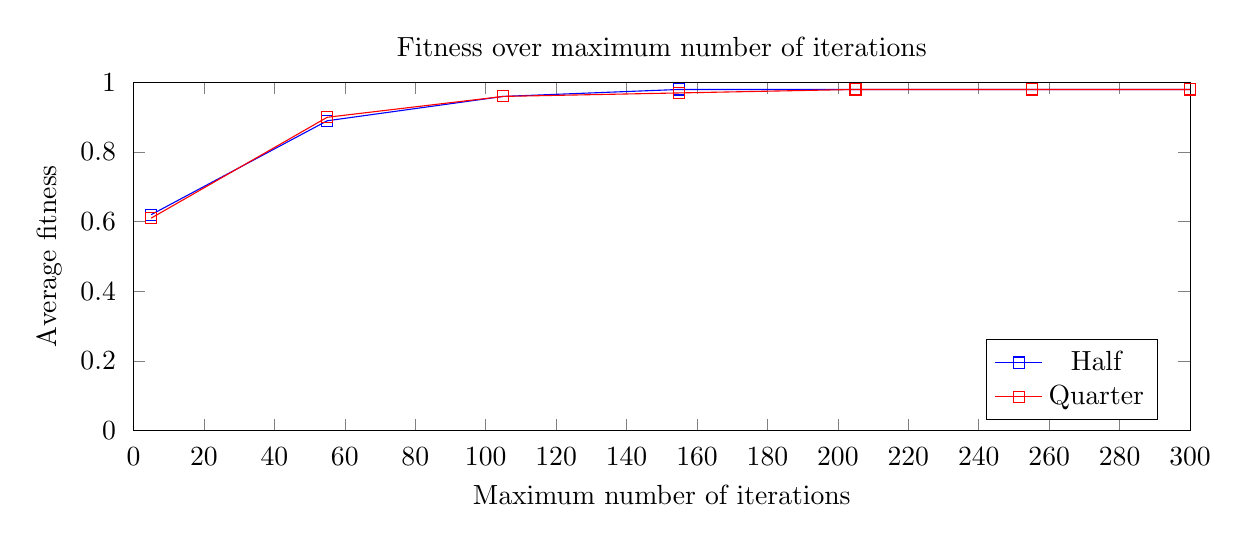
\begin{tikzpicture}
        \begin{axis}[
            width=15cm,
            height=6cm,
            title={Fitness over maximum number of iterations},
            legend pos=south east,
            xlabel={Maximum number of iterations},
            ylabel={Average fitness},
            enlargelimits=false,
            xmin=0,
            ymin=0, ymax=1,
            ytick={0,0.2,...,1},
            xticklabel shift={.1cm},
            yticklabel shift={.1cm} ]
        ]

        \addplot[
            color=blue,
            mark=square,
            ]
            coordinates {
                (5,0.62)(55,0.89)(105,0.96)(155,0.98)(205,0.98)(255,0.98)(300,0.98)
            };
            \addlegendentry{Half}
        \addplot[
            color=red,
            mark=square,
            ]
            coordinates {
                (5,0.61)(55,0.90)(105,0.96)(155,0.97)(205,0.98)(255,0.98)(300,0.98)
            };
            \addlegendentry{Quarter}
        \end{axis}
        \end{tikzpicture}
        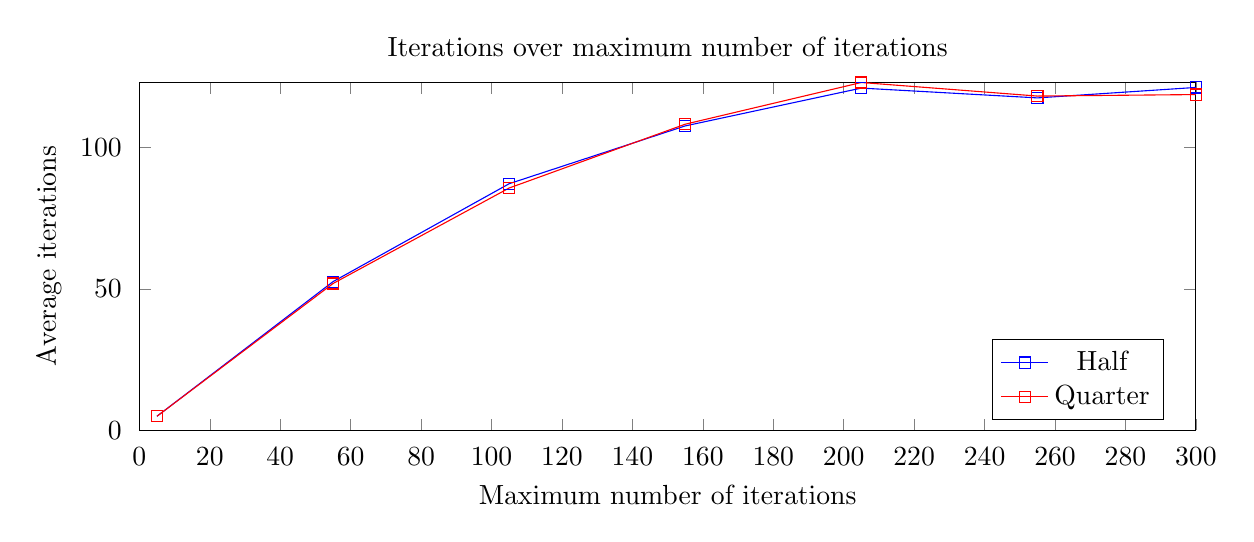
\begin{tikzpicture}
        \begin{axis}[
            width=15cm,
            height=6cm,
            legend pos=south east,
            title={Iterations over maximum number of iterations},
            xlabel={Maximum number of iterations},
            ylabel={Average iterations},
            xmin=0,
            ymin=0,
            enlargelimits=false,
            xticklabel shift={.1cm},
            yticklabel shift={.1cm} ]
        ]

        \addplot[
            color=blue,
            mark=square,
            ]
            coordinates {
                (5,5.00)(55,52.63)(105,87.26)(155,107.71)(205,121.09)(255,117.62)(300,121.32)
            };
            \addlegendentry{Half}
        \addplot[
            color=red,
            mark=square,
            ]
            coordinates {
                (5,5.00)(55,51.96)(105,85.74)(155,108.32)(205,123.07)(255,118.27)(300,118.80)
            };
            \addlegendentry{Quarter}
        \end{axis}
        \end{tikzpicture}
        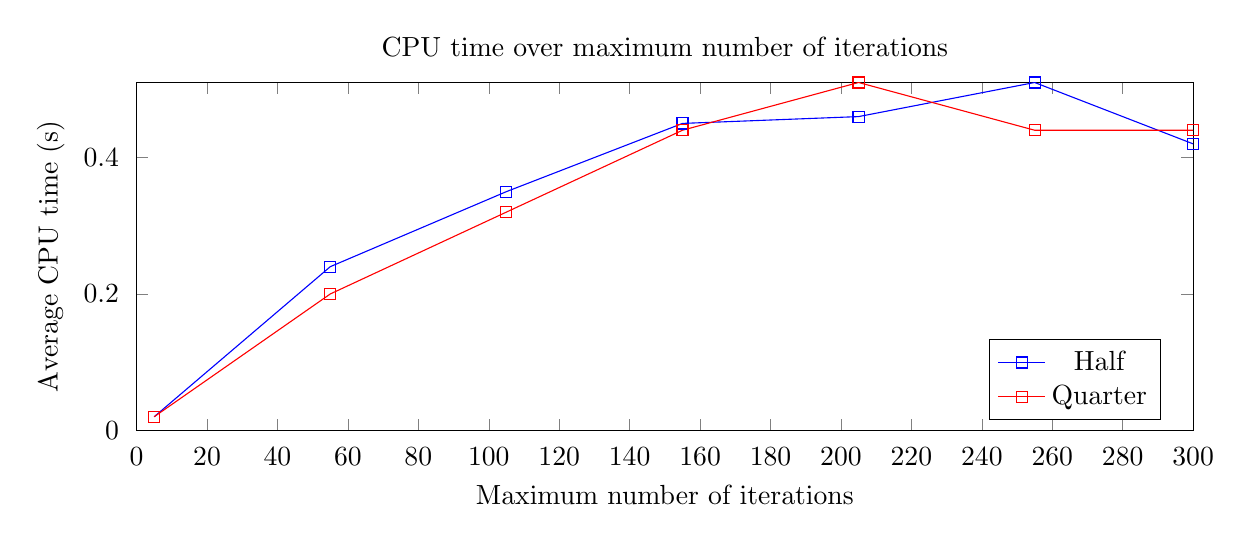
\begin{tikzpicture}
        \begin{axis}[
            width=15cm,
            height=6cm,
            legend pos=south east,
            title={CPU time over maximum number of iterations},
            xlabel={Maximum number of iterations},
            ylabel={Average CPU time (s)},
            xmin=0,
            ymin=0,
            enlargelimits=false,
            xticklabel shift={.1cm},
            yticklabel shift={.1cm} ]
        ]

        \addplot[
            color=blue,
            mark=square,
            ]
            coordinates {
                (5,0.02)(55,0.24)(105,0.35)(155,0.45)(205,0.46)(255,0.51)(300,0.42)
            };
            \addlegendentry{Half}
        \addplot[
            color=red,
            mark=square,
            ]
            coordinates {
                (5,0.02)(55,0.20)(105,0.32)(155,0.44)(205,0.51)(255,0.44)(300,0.44)
            };
            \addlegendentry{Quarter}
        \end{axis}
        \end{tikzpicture}
    \end{center}
    \caption{Performance metrics of the BNA algorithm on the \textit{Half} and \textit{Quarter} benchmarks, over different maximum iterations.
    The evolution stopped when the fitness was $2\%$ away from the maximal fitness of $1.0$ or the maximum number of iterations was reached.}
    \label{fig:bna_half_quarter}
\end{figure}

\begin{figure}
    \begin{center}
        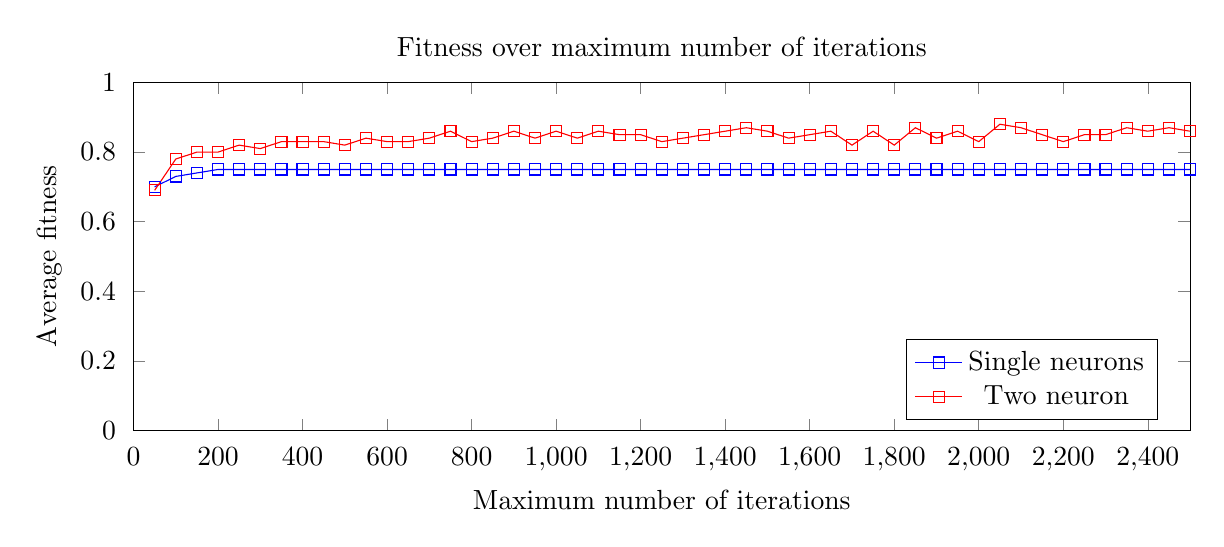
\begin{tikzpicture}
        \begin{axis}[
            width=15cm,
            height=6cm,
            title={Fitness over maximum number of iterations},
            legend pos=south east,
            xlabel={Maximum number of iterations},
            ylabel={Average fitness},
            enlargelimits=false,
            xmin=0,
            ymin=0, ymax=1,
            ytick={0,0.2,...,1},
            xticklabel shift={.1cm},
            yticklabel shift={.1cm} ]
        ]

        \addplot[
            color=blue,
            mark=square,
            ]
            coordinates {
(50,0.70)(100,0.73)(150,0.74)(200,0.75)(250,0.75)(300,0.75)(350,0.75)(400,0.75)(450,0.75)(500,0.75)(550,0.75)(600,0.75)(650,0.75)(700,0.75)(750,0.75)(800,0.75)(850,0.75)(900,0.75)(950,0.75)(1000,0.75)(1050,0.75)(1100,0.75)(1150,0.75)(1200,0.75)(1250,0.75)(1300,0.75)(1350,0.75)(1400,0.75)(1450,0.75)(1500,0.75)(1550,0.75)(1600,0.75)(1650,0.75)(1700,0.75)(1750,0.75)(1800,0.75)(1850,0.75)(1900,0.75)(1950,0.75)(2000,0.75)(2050,0.75)(2100,0.75)(2150,0.75)(2200,0.75)(2250,0.75)(2300,0.75)(2350,0.75)(2400,0.75)(2450,0.75)(2500,0.75)
            };
            \addlegendentry{Single neurons}
        \addplot[
            color=red,
            mark=square,
            ]
            coordinates {
(50,0.69)(100,0.78)(150,0.80)(200,0.80)(250,0.82)(300,0.81)(350,0.83)(400,0.83)(450,0.83)(500,0.82)(550,0.84)(600,0.83)(650,0.83)(700,0.84)(750,0.86)(800,0.83)(850,0.84)(900,0.86)(950,0.84)(1000,0.86)(1050,0.84)(1100,0.86)(1150,0.85)(1200,0.85)(1250,0.83)(1300,0.84)(1350,0.85)(1400,0.86)(1450,0.87)(1500,0.86)(1550,0.84)(1600,0.85)(1650,0.86)(1700,0.82)(1750,0.86)(1800,0.82)(1850,0.87)(1900,0.84)(1950,0.86)(2000,0.83)(2050,0.88)(2100,0.87)(2150,0.85)(2200,0.83)(2250,0.85)(2300,0.85)(2350,0.87)(2400,0.86)(2450,0.87)(2500,0.86)
            };
            \addlegendentry{Two neuron}
        \end{axis}
        \end{tikzpicture}
        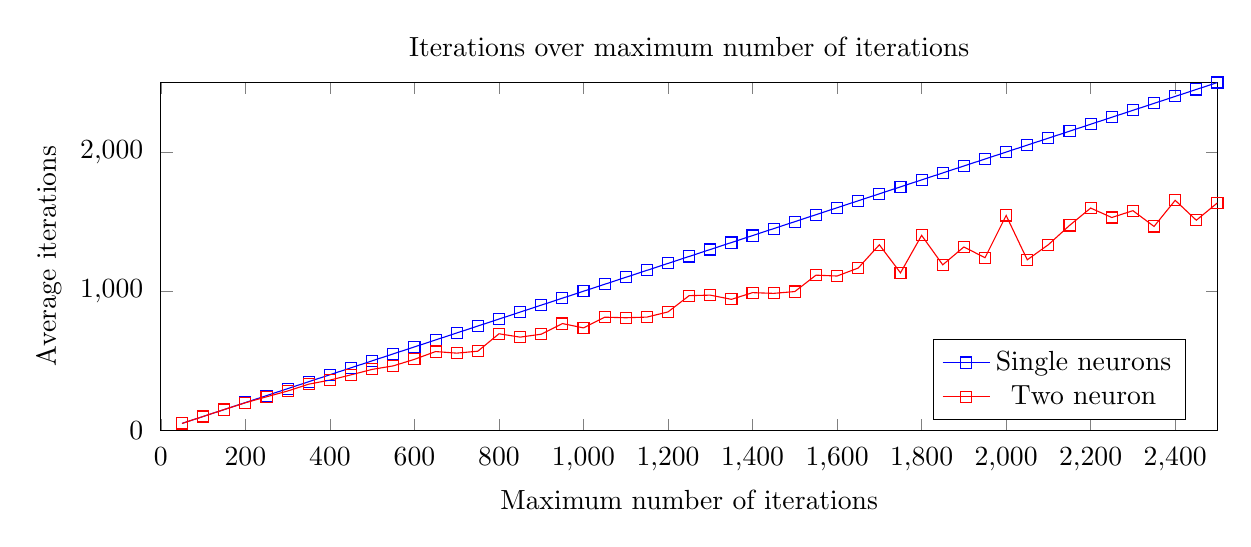
\begin{tikzpicture}
        \begin{axis}[
            width=15cm,
            height=6cm,
            legend pos=south east,
            title={Iterations over maximum number of iterations},
            xlabel={Maximum number of iterations},
            ylabel={Average iterations},
            xmin=0,
            ymin=0,
            enlargelimits=false,
            xticklabel shift={.1cm},
            yticklabel shift={.1cm} ]
        ]

        \addplot[
            color=blue,
            mark=square,
            ]
            coordinates {
(50,50.00)(100,100.00)(150,150.00)(200,200.00)(250,250.00)(300,300.00)(350,350.00)(400,400.00)(450,450.00)(500,500.00)(550,550.00)(600,600.00)(650,650.00)(700,700.00)(750,750.00)(800,800.00)(850,850.00)(900,900.00)(950,950.00)(1000,1000.00)(1050,1050.00)(1100,1100.00)(1150,1150.00)(1200,1200.00)(1250,1250.00)(1300,1300.00)(1350,1350.00)(1400,1400.00)(1450,1450.00)(1500,1500.00)(1550,1550.00)(1600,1600.00)(1650,1650.00)(1700,1700.00)(1750,1750.00)(1800,1800.00)(1850,1850.00)(1900,1900.00)(1950,1950.00)(2000,2000.00)(2050,2050.00)(2100,2100.00)(2150,2150.00)(2200,2200.00)(2250,2250.00)(2300,2300.00)(2350,2350.00)(2400,2400.00)(2450,2450.00)(2500,2500.00)
            };
            \addlegendentry{Single neurons}
        \addplot[
            color=red,
            mark=square,
            ]
            coordinates {
(50,50.00)(100,99.92)(150,150.00)(200,198.51)(250,241.50)(300,282.96)(350,332.40)(400,361.51)(450,399.29)(500,438.45)(550,463.70)(600,510.75)(650,566.58)(700,555.12)(750,569.20)(800,694.31)(850,670.17)(900,691.26)(950,767.70)(1000,736.54)(1050,813.48)(1100,809.46)(1150,814.14)(1200,851.38)(1250,968.46)(1300,972.02)(1350,941.72)(1400,989.87)(1450,984.70)(1500,997.75)(1550,1115.48)(1600,1109.32)(1650,1166.71)(1700,1333.93)(1750,1132.14)(1800,1401.49)(1850,1189.76)(1900,1318.19)(1950,1240.79)(2000,1544.52)(2050,1225.65)(2100,1334.69)(2150,1472.85)(2200,1597.69)(2250,1529.85)(2300,1578.75)(2350,1465.73)(2400,1653.33)(2450,1510.16)(2500,1635.20)
            };
            \addlegendentry{Two neuron}
        \end{axis}
        \end{tikzpicture}
        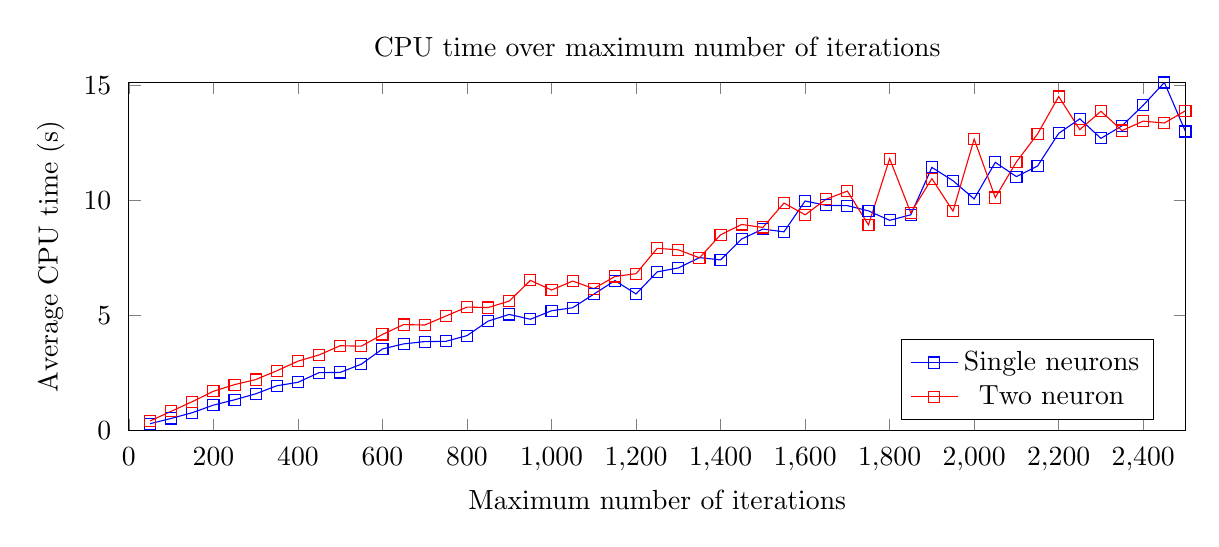
\begin{tikzpicture}
        \begin{axis}[
            width=15cm,
            height=6cm,
            legend pos=south east,
            title={CPU time over maximum number of iterations},
            xlabel={Maximum number of iterations},
            ylabel={Average CPU time (s)},
            xmin=0,
            ymin=0,
            enlargelimits=false,
            xticklabel shift={.1cm},
            yticklabel shift={.1cm} ]
        ]

        \addplot[
            color=blue,
            mark=square,
            ]
            coordinates {
(50,0.29)(100,0.52)(150,0.77)(200,1.10)(250,1.33)(300,1.59)(350,1.94)(400,2.09)(450,2.51)(500,2.52)(550,2.88)(600,3.54)(650,3.76)(700,3.86)(750,3.87)(800,4.12)(850,4.75)(900,5.04)(950,4.83)(1000,5.20)(1050,5.33)(1100,5.92)(1150,6.51)(1200,5.93)(1250,6.89)(1300,7.06)(1350,7.51)(1400,7.41)(1450,8.32)(1500,8.75)(1550,8.63)(1600,9.97)(1650,9.78)(1700,9.77)(1750,9.54)(1800,9.13)(1850,9.37)(1900,11.43)(1950,10.85)(2000,10.06)(2050,11.65)(2100,11.03)(2150,11.49)(2200,12.91)(2250,13.54)(2300,12.69)(2350,13.24)(2400,14.13)(2450,15.12)(2500,12.99)
            };
            \addlegendentry{Single neurons}
        \addplot[
            color=red,
            mark=square,
            ]
            coordinates {
(50,0.41)(100,0.83)(150,1.25)(200,1.70)(250,1.99)(300,2.21)(350,2.59)(400,3.01)(450,3.28)(500,3.68)(550,3.66)(600,4.17)(650,4.60)(700,4.58)(750,4.97)(800,5.36)(850,5.34)(900,5.62)(950,6.52)(1000,6.10)(1050,6.49)(1100,6.16)(1150,6.69)(1200,6.81)(1250,7.91)(1300,7.85)(1350,7.50)(1400,8.50)(1450,8.95)(1500,8.82)(1550,9.88)(1600,9.37)(1650,10.05)(1700,10.40)(1750,8.93)(1800,11.81)(1850,9.46)(1900,10.94)(1950,9.53)(2000,12.66)(2050,10.12)(2100,11.67)(2150,12.88)(2200,14.51)(2250,13.07)(2300,13.87)(2350,13.03)(2400,13.44)(2450,13.36)(2500,13.89)
            };
            \addlegendentry{Two neuron}
        \end{axis}
        \end{tikzpicture}
    \end{center}
    \caption{Performance metrics of the BNA algorithm on the \textit{TwoQuarters} benchmark, over different maximum iterations.
    The evolution stopped when the fitness was $2\%$ away from the maximal fitness of $1.0$ or the maximum number of iterations was reached.}
    \label{fig:bna_twoquarters}
\end{figure}

\begin{figure}
    \begin{center}
        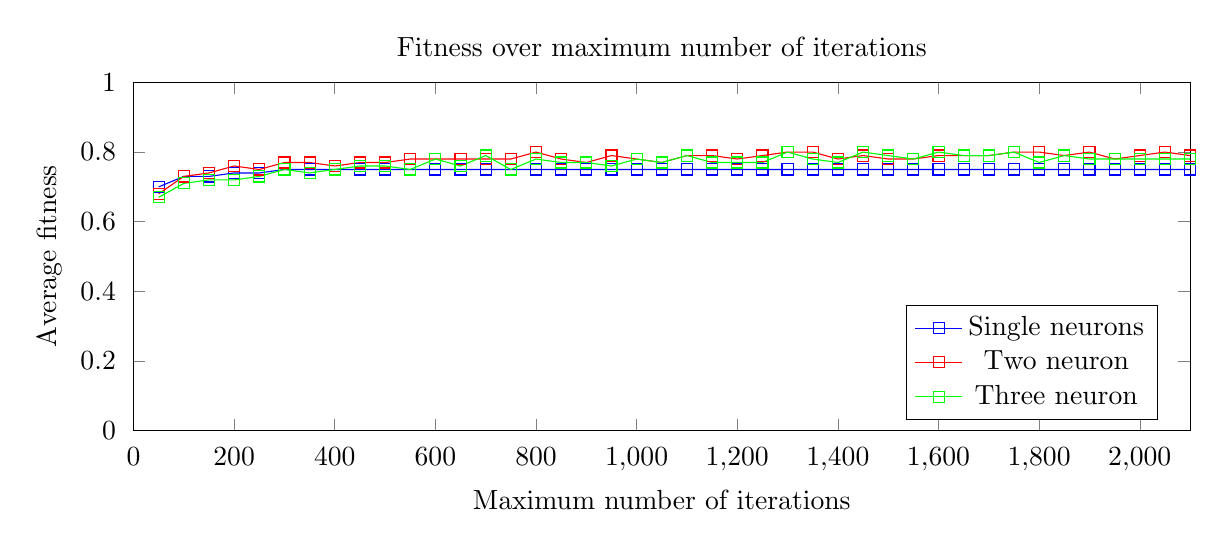
\begin{tikzpicture}
        \begin{axis}[
            width=15cm,
            height=6cm,
            title={Fitness over maximum number of iterations},
            legend pos=south east,
            xlabel={Maximum number of iterations},
            ylabel={Average fitness},
            enlargelimits=false,
            xmin=0,
            ymin=0, ymax=1,
            ytick={0,0.2,...,1},
            xticklabel shift={.1cm},
            yticklabel shift={.1cm} ]
        ]

        \addplot[
            color=blue,
            mark=square,
            ]
            coordinates {
                (50,0.70)(100,0.73)(150,0.73)(200,0.74)(250,0.74)(300,0.75)(350,0.75)(400,0.75)(450,0.75)(500,0.75)(550,0.75)(600,0.75)(650,0.75)(700,0.75)(750,0.75)(800,0.75)(850,0.75)(900,0.75)(950,0.75)(1000,0.75)(1050,0.75)(1100,0.75)(1150,0.75)(1200,0.75)(1250,0.75)(1300,0.75)(1350,0.75)(1400,0.75)(1450,0.75)(1500,0.75)(1550,0.75)(1600,0.75)(1650,0.75)(1700,0.75)(1750,0.75)(1800,0.75)(1850,0.75)(1900,0.75)(1950,0.75)(2000,0.75)(2050,0.75)(2100,0.75)
            };
            \addlegendentry{Single neurons}
        \addplot[
            color=red,
            mark=square,
            ]
            coordinates {
                (50,0.68)(100,0.73)(150,0.74)(200,0.76)(250,0.75)(300,0.77)(350,0.77)(400,0.76)(450,0.77)(500,0.77)(550,0.78)(600,0.78)(650,0.78)(700,0.78)(750,0.78)(800,0.80)(850,0.78)(900,0.77)(950,0.79)(1000,0.78)(1050,0.77)(1100,0.79)(1150,0.79)(1200,0.78)(1250,0.79)(1300,0.80)(1350,0.80)(1400,0.78)(1450,0.79)(1500,0.78)(1550,0.78)(1600,0.79)(1650,0.79)(1700,0.79)(1750,0.80)(1800,0.80)(1850,0.79)(1900,0.80)(1950,0.78)(2000,0.79)(2050,0.80)(2100,0.79)
            };
            \addlegendentry{Two neuron}
        \addplot[
            color=green,
            mark=square,
            ]
            coordinates {
                (50,0.67)(100,0.71)(150,0.72)(200,0.72)(250,0.73)(300,0.75)(350,0.74)(400,0.75)(450,0.76)(500,0.76)(550,0.75)(600,0.78)(650,0.76)(700,0.79)(750,0.75)(800,0.78)(850,0.77)(900,0.77)(950,0.76)(1000,0.78)(1050,0.77)(1100,0.79)(1150,0.77)(1200,0.77)(1250,0.77)(1300,0.80)(1350,0.78)(1400,0.77)(1450,0.80)(1500,0.79)(1550,0.78)(1600,0.80)(1650,0.79)(1700,0.79)(1750,0.80)(1800,0.77)(1850,0.79)(1900,0.78)(1950,0.78)(2000,0.78)(2050,0.78)(2100,0.78)
            };
            \addlegendentry{Three neuron}
        \end{axis}
        \end{tikzpicture}
        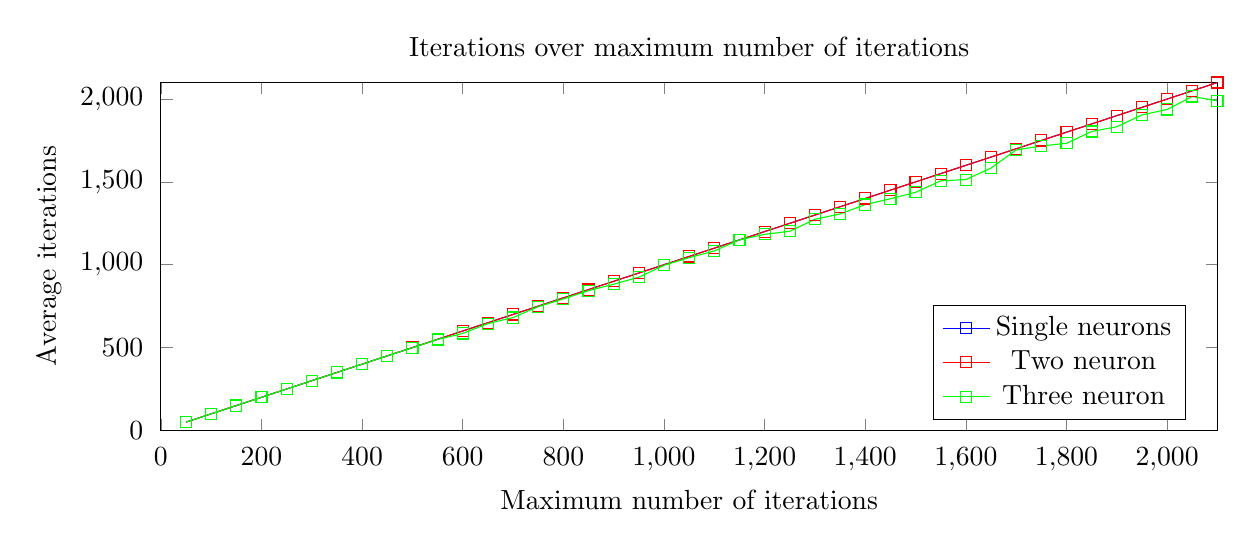
\begin{tikzpicture}
        \begin{axis}[
            width=15cm,
            height=6cm,
            legend pos=south east,
            title={Iterations over maximum number of iterations},
            xlabel={Maximum number of iterations},
            ylabel={Average iterations},
            xmin=0,
            ymin=0,
            enlargelimits=false,
            xticklabel shift={.1cm},
            yticklabel shift={.1cm} ]
        ]

        \addplot[
            color=blue,
            mark=square,
            ]
            coordinates {
                (50,50.00)(100,100.00)(150,150.00)(200,200.00)(250,250.00)(300,300.00)(350,350.00)(400,400.00)(450,450.00)(500,500.00)(550,550.00)(600,600.00)(650,650.00)(700,700.00)(750,750.00)(800,800.00)(850,850.00)(900,900.00)(950,950.00)(1000,1000.00)(1050,1050.00)(1100,1100.00)(1150,1150.00)(1200,1200.00)(1250,1250.00)(1300,1300.00)(1350,1350.00)(1400,1400.00)(1450,1450.00)(1500,1500.00)(1550,1550.00)(1600,1600.00)(1650,1650.00)(1700,1700.00)(1750,1750.00)(1800,1800.00)(1850,1850.00)(1900,1900.00)(1950,1950.00)(2000,2000.00)(2050,2050.00)(2100,2100.00)
            };
            \addlegendentry{Single neurons}
        \addplot[
            color=red,
            mark=square,
            ]
            coordinates {
                (50,50.00)(100,100.00)(150,150.00)(200,200.00)(250,250.00)(300,300.00)(350,350.00)(400,400.00)(450,450.00)(500,500.00)(550,550.00)(600,600.00)(650,650.00)(700,700.00)(750,750.00)(800,800.00)(850,850.00)(900,900.00)(950,950.00)(1000,1000.00)(1050,1050.00)(1100,1100.00)(1150,1150.00)(1200,1200.00)(1250,1250.00)(1300,1300.00)(1350,1350.00)(1400,1400.00)(1450,1450.00)(1500,1500.00)(1550,1550.00)(1600,1600.00)(1650,1650.00)(1700,1700.00)(1750,1750.00)(1800,1800.00)(1850,1850.00)(1900,1900.00)(1950,1950.00)(2000,2000.00)(2050,2050.00)(2100,2100.00)
            };
            \addlegendentry{Two neuron}
        \addplot[
            color=green,
            mark=square,
            ]
            coordinates {
                (50,50.00)(100,100.00)(150,150.00)(200,200.00)(250,250.00)(300,300.00)(350,350.00)(400,400.00)(450,450.00)(500,498.69)(550,548.75)(600,585.31)(650,644.70)(700,681.21)(750,746.81)(800,793.97)(850,843.65)(900,882.82)(950,924.71)(1000,996.55)(1050,1042.52)(1100,1083.37)(1150,1150.00)(1200,1183.52)(1250,1202.19)(1300,1274.40)(1350,1306.74)(1400,1363.23)(1450,1397.99)(1500,1437.08)(1550,1506.49)(1600,1513.89)(1650,1583.68)(1700,1693.09)(1750,1716.86)(1800,1732.89)(1850,1804.30)(1900,1832.85)(1950,1904.38)(2000,1937.28)(2050,2015.75)(2100,1988.72)
            };
            \addlegendentry{Three neuron}
        \end{axis}
        \end{tikzpicture}
        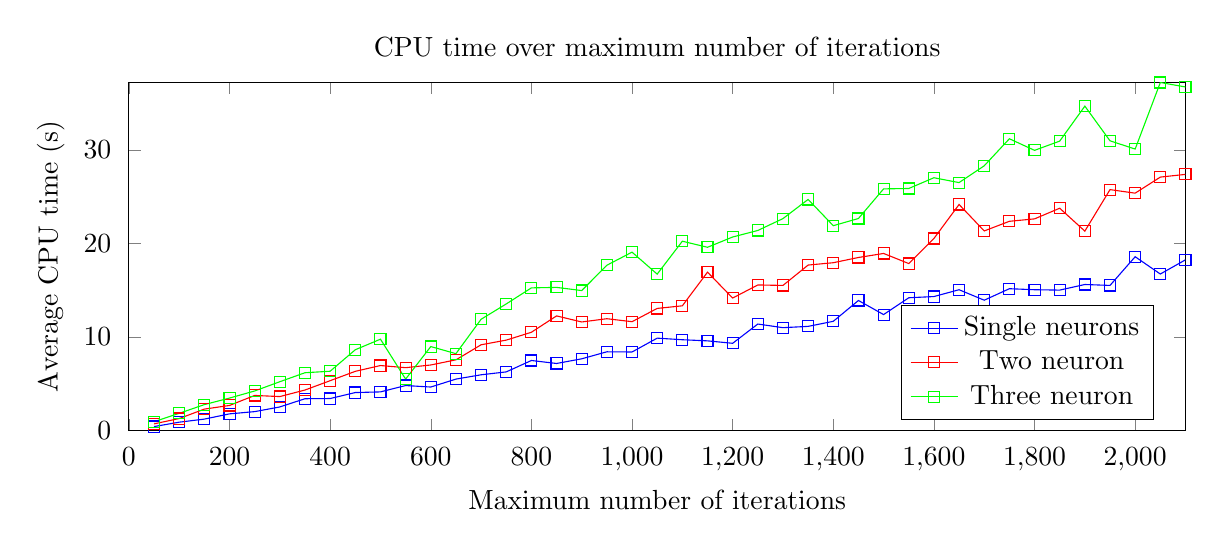
\begin{tikzpicture}
        \begin{axis}[
            width=15cm,
            height=6cm,
            legend pos=south east,
            title={CPU time over maximum number of iterations},
            xlabel={Maximum number of iterations},
            ylabel={Average CPU time (s)},
            xmin=0,
            ymin=0,
            enlargelimits=false,
            xticklabel shift={.1cm},
            yticklabel shift={.1cm} ]
        ]

        \addplot[
            color=blue,
            mark=square,
            ]
            coordinates {
                (50,0.41)(100,0.88)(150,1.21)(200,1.77)(250,2.01)(300,2.51)(350,3.39)(400,3.41)(450,4.05)(500,4.12)(550,4.80)(600,4.64)(650,5.49)(700,5.95)(750,6.26)(800,7.48)(850,7.16)(900,7.66)(950,8.41)(1000,8.39)(1050,9.87)(1100,9.70)(1150,9.58)(1200,9.32)(1250,11.38)(1300,10.99)(1350,11.13)(1400,11.67)(1450,13.90)(1500,12.39)(1550,14.19)(1600,14.32)(1650,15.05)(1700,13.93)(1750,15.16)(1800,15.05)(1850,15.01)(1900,15.61)(1950,15.51)(2000,18.58)(2050,16.73)(2100,18.25)
            };
            \addlegendentry{Single neurons}
        \addplot[
            color=red,
            mark=square,
            ]
            coordinates {
                (50,0.70)(100,1.27)(150,2.28)(200,2.67)(250,3.74)(300,3.62)(350,4.32)(400,5.32)(450,6.32)(500,6.94)(550,6.71)(600,7.00)(650,7.55)(700,9.16)(750,9.66)(800,10.50)(850,12.25)(900,11.60)(950,11.95)(1000,11.63)(1050,13.05)(1100,13.33)(1150,16.93)(1200,14.16)(1250,15.56)(1300,15.51)(1350,17.69)(1400,17.94)(1450,18.50)(1500,18.93)(1550,17.85)(1600,20.53)(1650,24.17)(1700,21.34)(1750,22.37)(1800,22.63)(1850,23.77)(1900,21.32)(1950,25.76)(2000,25.38)(2050,27.10)(2100,27.39)
            };
            \addlegendentry{Two neuron}
        \addplot[
            color=green,
            mark=square,
            ]
            coordinates {
                (50,0.93)(100,1.83)(150,2.76)(200,3.46)(250,4.22)(300,5.21)(350,6.17)(400,6.33)(450,8.63)(500,9.76)(550,5.49)(600,8.97)(650,8.21)(700,11.89)(750,13.53)(800,15.25)(850,15.30)(900,14.96)(950,17.67)(1000,19.07)(1050,16.72)(1100,20.24)(1150,19.59)(1200,20.69)(1250,21.39)(1300,22.66)(1350,24.71)(1400,21.90)(1450,22.67)(1500,25.84)(1550,25.88)(1600,27.03)(1650,26.51)(1700,28.31)(1750,31.20)(1800,29.96)(1850,30.95)(1900,34.69)(1950,30.98)(2000,30.10)(2050,37.22)(2100,36.74)
            };
            \addlegendentry{Three neuron}
        \end{axis}
        \end{tikzpicture}
    \end{center}
    \caption{Performance metrics of the BNA algorithm on the \textit{LocalOpt} benchmark, over different maximum iterations.
    The evolution stopped when the fitness was $2\%$ away from the maximal fitness of $1.0$ or the maximum number of iterations was reached.}
    \label{fig:bna_localopt}
\end{figure}

\subsection{Results of the NEAT algorithm}

...

\subsection{Results of the CMA-ES algorithm}

...
